\chapter{Common analysis components}
\label{chap:common_analysis_components}
\chapterquote{I don't have a quote}
{Matthew Kenzie, 1785--1854}

This thesis describes three complementary analysis regimes in the Higgs to two photons search at CMS. These differ in their photon selection, event selection, event classification (or categorisation) and statistical methods for extracting results. They are described in the following chapter (Chapter~\ref{chap:selection_and_categorisation}). However, there are many components which they share. These are detailed below.

As we have seen in Eq.~\ref{eq:invmass}, repeated below in Eq.~\ref{eq:invmass2} for convenience, the diphoton invariant mass is constructed from the two photon energies and the angle between them. Consequently, important considerations for this analysis are photon energy resolution and good opening angle resolution which is compltely dominanted by the vertex resolution as the position resolution of the photons (location they hit the \ECAL) is neglible in comparison. Details of how this is exploited in the analyses are given at the end of this chapter in Sections~\ref{sec:photon_energy} and~\ref{sec:vtx_reco}. The selection of events is described in the chapter after this (Chapter~\ref{chap:selection_and_categorisation}) alongside the categorisation, or binning, scheme into different classes of event which take advantage of areas of phase space with different signal to background ratios.

\begin{equation}
  m_{\gamma\gamma} = \sqrt{E_{1}E_{2}(1-\cos(\alpha))}
  \label{eq:invmass2}
\end{equation}

After a preliminary discussion of multivariate analysis techniques, the datasets, the triggering and the \MC are discussed.

\section{Boosted Decision Trees}
\label{sec:bdts}

\MVAs are commonly used in High Energy Physics analyses to extract the maximum possible signal sensitivity in cases where the background rates are high. The advantage of \MVAs is that given a set of input variables a network of sequential cuts can be built in a multidimensional phase space to exploit differences between the signal and background in these variables and importantly in the correlations between these variables. A particular type of \MVA which is used widely in this analysis is the \BDT. \BDTs are preffered because they are more robust to the inclusion of variables which have little or no discriminating power. There are two broad types of \BDT used, one is known as a regression \BDT and the other as a classification \BDT. 

A classification \BDT will assign a value (typically between -1 and 1) to each event based on how signal like that event is which serves to collapse all the event information into one discrimanting variable which can be used to classify differences between the signal and background. The input is provided as the probability distributions (which can be provided as a binned or unbinned data sample or a functional form) of the background and signal for a set of ``input variables". The process involves construction of a series of \DTs complemented by a ``boosting" step which serves to mitigate against ``overtraining" on fluctuations within the training samples. This analysis chooses a particular type of decision tree boosting known as ``gradient" boosting because it is more robust against outliers or mislabled data points~\cite{TMVA}.

The \DT is built by applying sequential cuts to the input variables and assessing the relative signal purity, $p$, in the sub-sample remaining after each cut.

\begin{equation}
  p = \frac{N_{s}}{N_{s}+N_{b}},
\end{equation}

where $N_{s}$ and $N_{b}$ are the sum of weights of the signal and background remaining in each sub-sample. A threshold criterion, known as the Gini index~\cite{TMVA} $p(1-p)$, is applied to decide whether to split the sample further. The process continues and the splitting is curtailed when either the threshold or the user defined maximum tree depth (number of subsamples allowed) is reached. The value of each cut is varied such that the signal purity, $p$, in each sub-sample is maximised. An event is assigned a value of -1 or +1 depending on whether it falls into a sub-sample with $p$>0.5 or not. Claerly some fraction of events will be missclassifed where the actual number which get missclassified will depend on the discrimnatory power available from the chosen input variables. In order to reduce this effect a series of \DTs are trained and each assigned a weight derived by the ``boosting" process. 
If we assign each \DT as a member of a family of $M$ functions, $f(\vec{x};\vec{a}_{m})$, which are depend on the input variables, $\vec{x}$ and the set of cuts in that tree $\vec{a}=\vec{a}_{m}$. The object is to construct an overall decision tree which consists of the weighted average of each \DT,

\begin{equation}
  F(\vec{x};\vec{\beta},\vec{a}) = \sum_{m=0}^{M} \beta_{m}f(\vec{x},\vec{a}_{m}) \;\;\;\;\; \textrm{where} \;\; \vec{\beta} = (\beta_{0},\beta_{1}...\beta_{m})
\end{equation}

The boosting procedue is implemented by adjusting the weights $\beta_{m}$ in order to minimise the deviation in the loss function (Eq.~\ref{eq:bdt_loss_fcn}) between the weighted tree response $F(\vec{x};\vec{\beta},\vec{a})$ and the true output $y$ obtained from the training sample. 

A common procedure when constructing a \BDT to check for overtraining is to split both the background and signal into two independent samples. One is used to \emph{train} the \BDT and one is used to \emph{test} the response of the output. Clearly one requires that both the training and independent test sample look the same in the output variable. This can be quantified by use of a Kolgomorov-Smirnoff test (\refrqd). 

\begin{equation}
  L(F,y) = \ln(1+e^{-2F(x)y})
  \label{eq:bdt_loss_fcn}
\end{equation}

In this way the output of $F(\vec{x};\vec{\beta},\vec{a})$ for a classification \BDT will be a ``semi-continuous" output from -1 to 1 with signal events in general given a higher score than background events.

A regression \BDT is used to derive the true value of some variable given the values and correlations of several other variables. They are commonly used for correcting the energy of a particular object, for example a photon. Given a \MC source of photons the ``true" energy is regressed from the position, shape and raw energy of the supercluster. For regression \BDTs the output $F(\vec{x};\vec{\beta},\vec{a})$ represents the estimated corrected energy and the boosting procedure targets minimising the deviation between this and the true energy in \MC. 

\section{Data samples and triggering}

The data consists of two indepedent samples of proton-proton collisions collected by the CMS experiment at the \LHC in 2011 and 2012 with a centre-of-mass energy ($\sqrt{s}$) of 7 and 8 TeV respecivtely. The total integrated luminosity of the two samples is 5.1\fb and 19.7\fb in 2011 and 2012 respectively and collectively referred to as \LHC Run 1. The response of the detector has changed considerably over this period and much of the variation is modelled by the \MC simulation. Figure~\ref{fig:intlumi} shows the integrated luminosity delivered and recorded by \CMS during \LHC Run 1.

\begin{figure}
  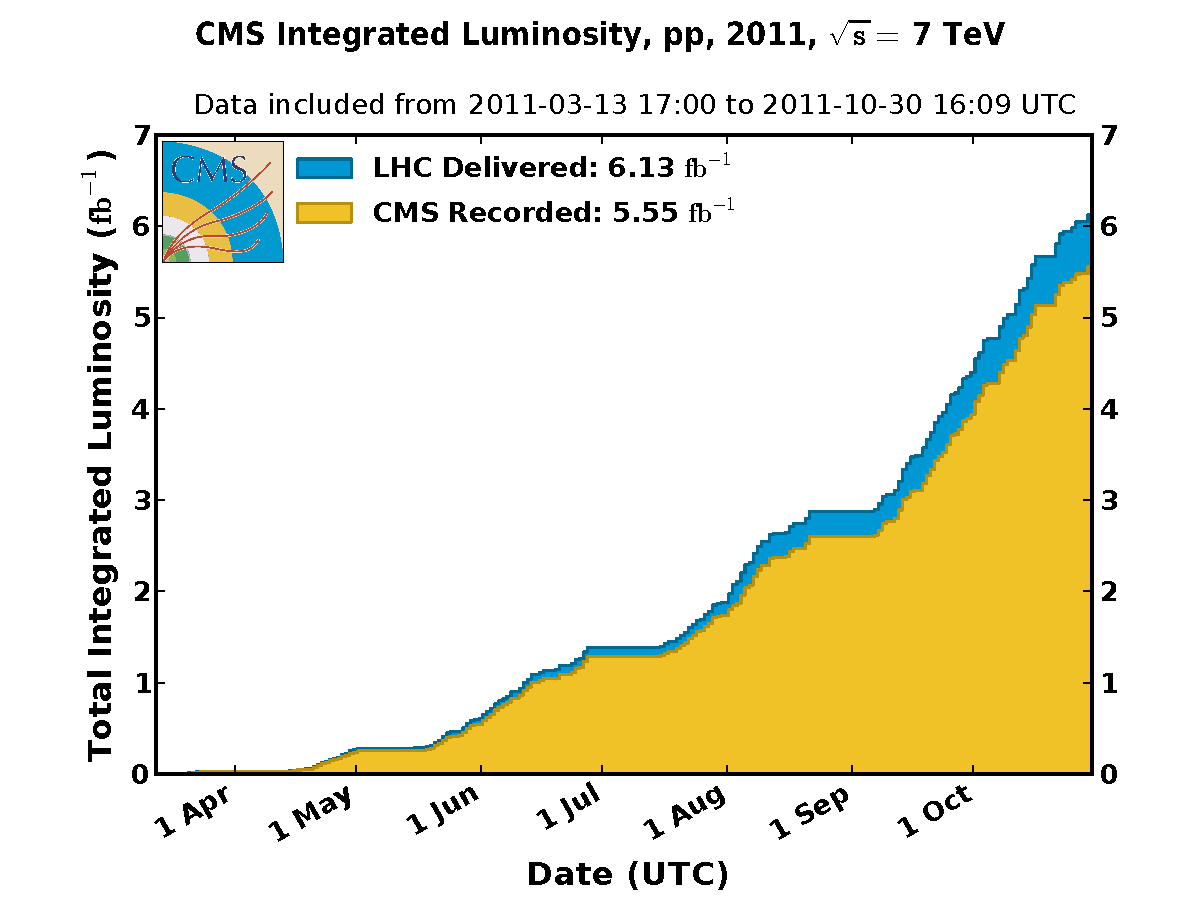
\includegraphics[width=0.49\textwidth]{ch3_comm_anal_comps/plots/int_lumi_2011.pdf}
  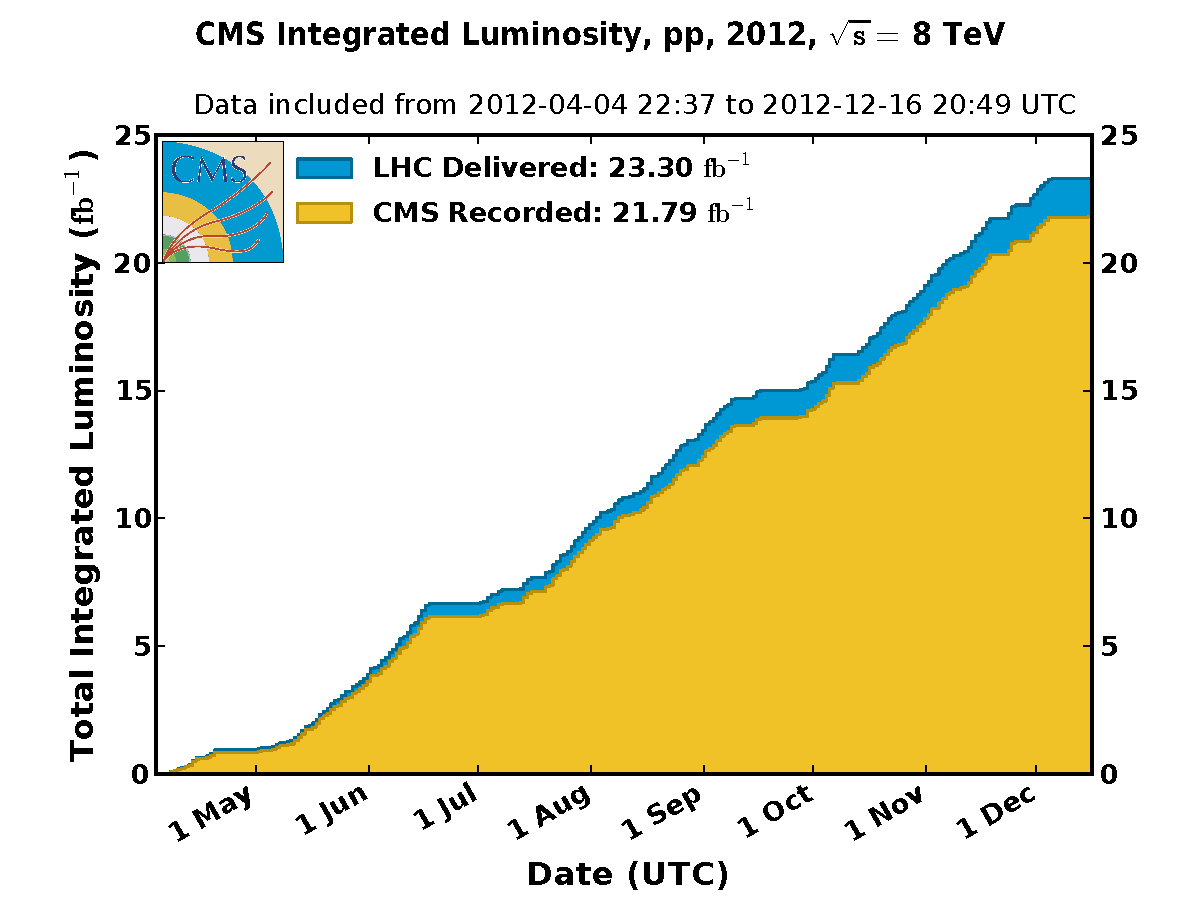
\includegraphics[width=0.49\textwidth]{ch3_comm_anal_comps/plots/int_lumi_2012.pdf}
  \caption{The total integrated luminosity delived and recorded by CMS during the 2011 (left) and 2012 (right) run periods.}
  \label{fig:intlumi}
\end{figure}

Events are selected for the analysis by requiring they pass an asymmetric diphoton trigger with \ET thresholds of 26 (18) and 36 (22) GeV for the leading (trailing) photon in the 2011 and 2012 runs respectively. The triggering has further requirements on photon selection. The candidates are required to have either a high value of \rnine or to pass a loose calorimetric identifaction and isolation requirement. High trigger efficiency is achieved by selecting photon candidates which pass either requirement. The effiency of the trigger for the analysis preselection is 99.5\%.

\subsection{Monte Carlo}

Accurate simulation of detector effects and efficiency is highly important. Knowledge of the expected Higgs signal shape is clearly essential and although the size and shape of the \mgg background is entirely data driven when extracting results, simultaing the kinematics, shower shape and resolution properties of the background is essential when training the selection and optimising the binning. 

As explained in Section~\ref{sec:intro} the two main production mechanisms for a \SM Higgs boson at the \LHC are gluon fusion ($ggH$) and vector boson fusion ($qqH$). Typically the latter is produced at much higher Higgs \pT and this feature is exploited in the analysis. Consequently, it is important to model the \pT distribution of these two production modes accurately. The signal samples for these two processes are generated using \POWHEG \refrqd at NLO interfaced with \PYTHIA \refrqd including a reweighting factor which matches their \pT spectrum to that when including the NNLO and NNLL terms. For the associated production modes (with a $W^{\pm}$,$Z$ or $t$'s) only \PYTHIA is used.

The spin-2 graviton with minimal couplings, \graviton, has two production mechanisms, one via gluon-fusion ($ggX$) and one via quark-antiquark annihilation ($q\bar{q}X$). The graviton samples are generated using the \JHU generator \refrqd in which the \pT spectrum of these samples is matched to the SM so that any bias obtained from mismodelling of the $\pT$ is avoided.

The simulated background samples are used soley for cut and category optimisations and training of multivariate discriminants. The background which contains the \QCD continuum of prompt photons (refering back to Chapter~\ref{chap:intro} these are produced by Born and Box diagrams) is simulated using \SHERPA at 8\TeV and \MADGRAPH at 7\TeV. The prompt-fake and fake-fake backgrounds, in which one or more photons are faked by a neutral meson (usually a \pizero) reconstructed as a jet are generated using \PYTHIA. Samples of \Zee, \Zmumu and \Zmumugamma used for data/MC comparisons are generated with \POWHEG.

All of these \emph{generator level} samples are then run through the full \CMS detector simulation using \GEANT \refrqd. This includes the effect of overlapping vertices (pileup) and detector effects (such as noise and crystal degredation) in four bins of time (Run2011, Run2012AB, Run2012C, Run2012D).


\subsection{Pileup and beamspot reweighting}
\label{sec:pileup_beamspot}

An important difference between the simulated samples and the data which can have a large impact on the analysis is the distribution of the number of primary vertices. The \emph{pileup} in the event effects many important analysis variables, for example photon shower shape and photon isolation as well as the diphoton invariant mass if the chosen vertex is wrong. Consequently the \MC is reweighted such that the pileup distribution matches that in data. The reweighting technique is validated using \Zmumu events as shown in Figure~\ref{fig:pileup} for the 7 and 8\TeV samples respectively. 

\begin{figure}
  \begin{center}
  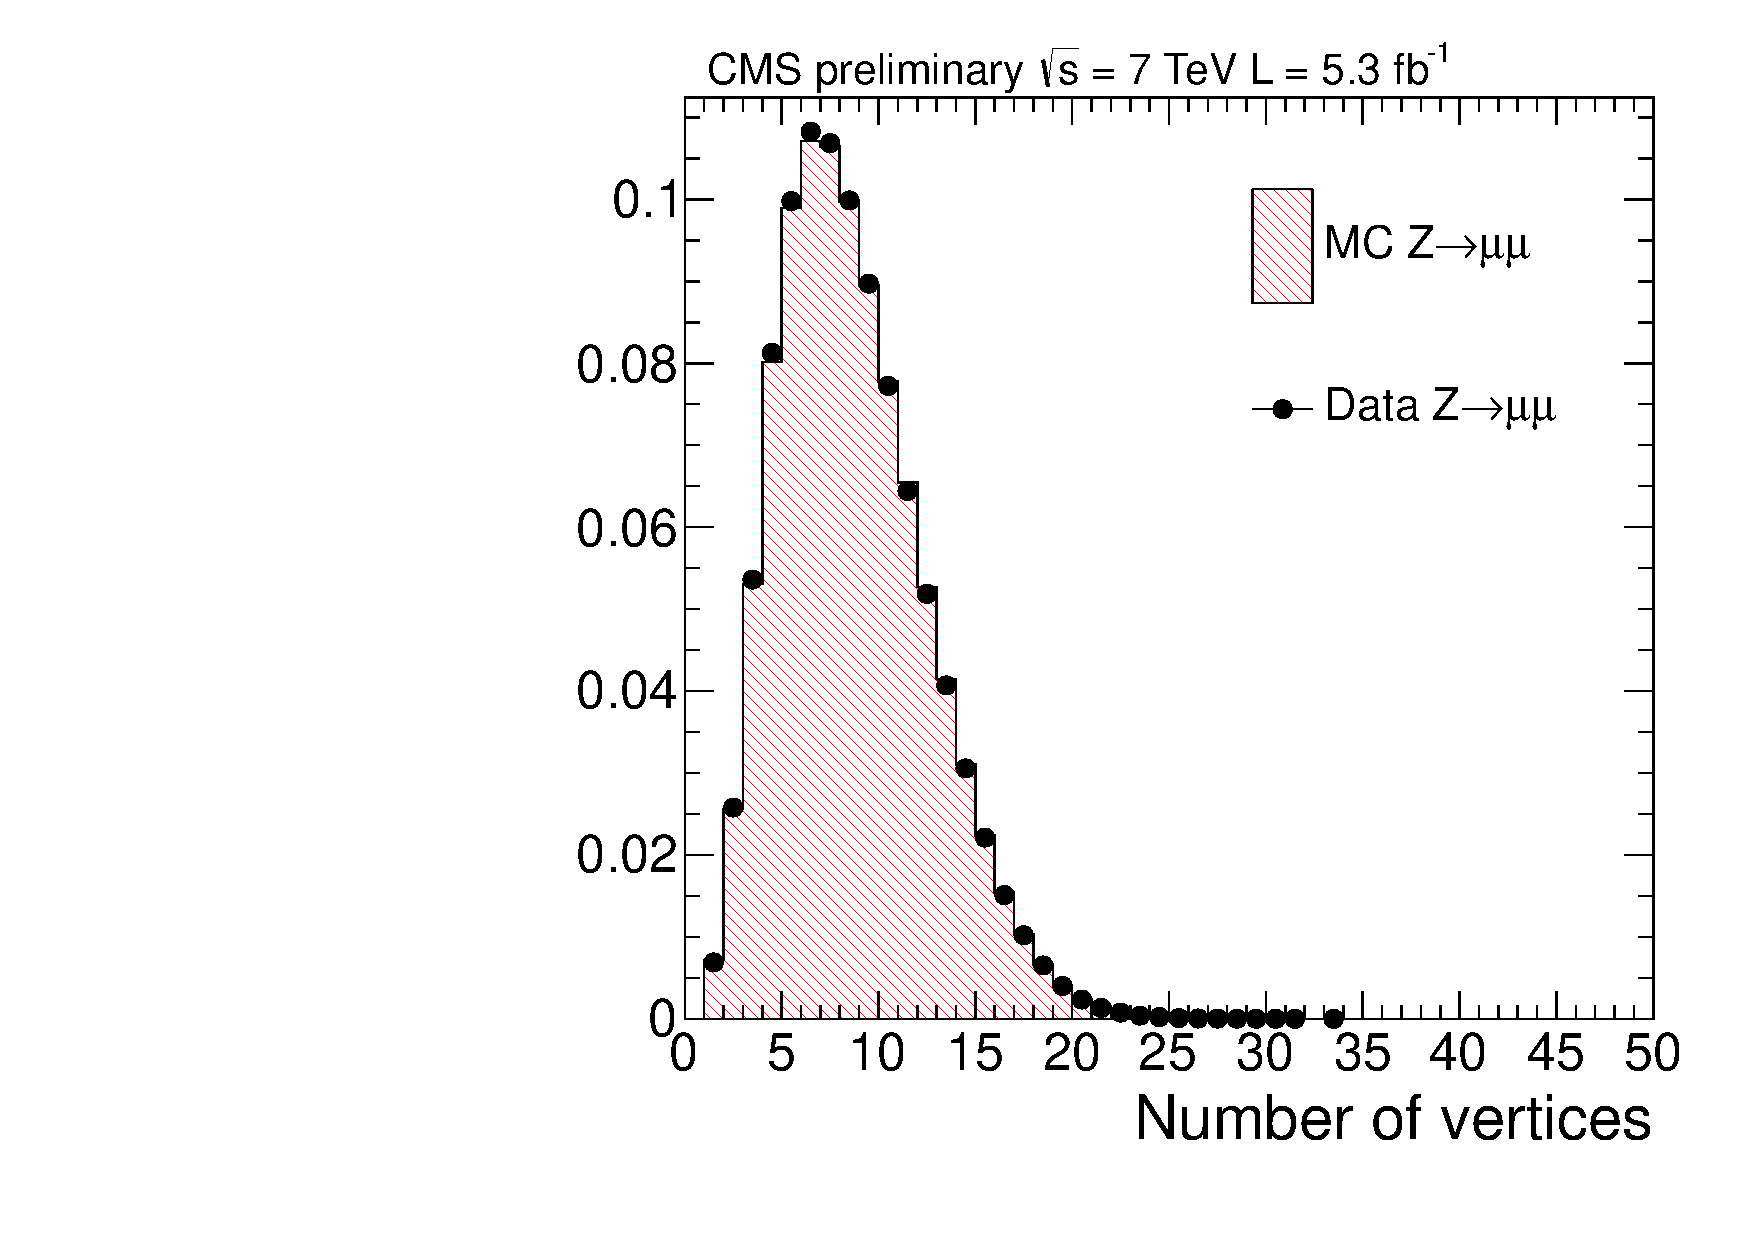
\includegraphics[width=0.49\textwidth]{ch3_comm_anal_comps/plots/nvtx_zmumu_2011.pdf}
  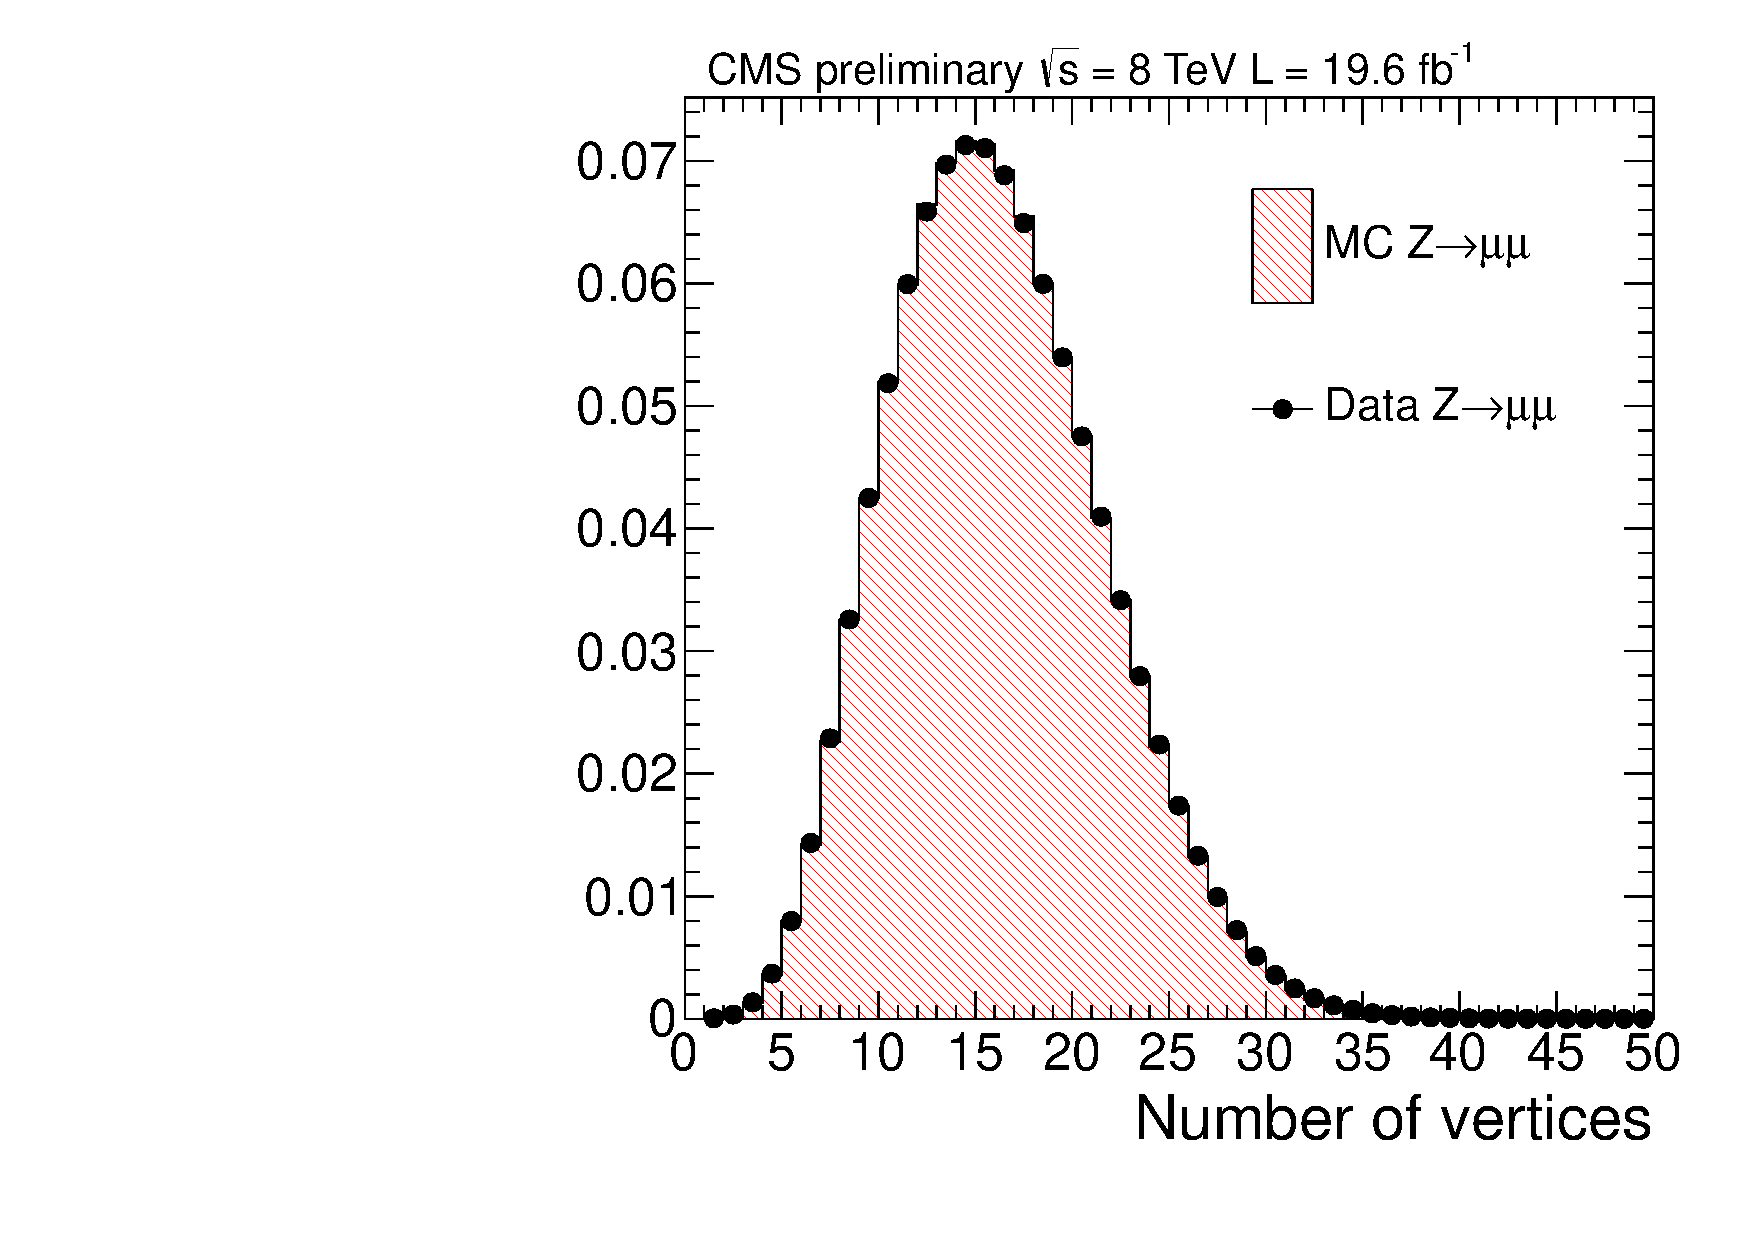
\includegraphics[width=0.49\textwidth]{ch3_comm_anal_comps/plots/nvtx_zmumu_2012.pdf}
  \caption{Distribution of the number of reconstructed vertices in the 2011 (left) and 2012 (right) run periods. Calculated using the Deterministic Annealing alogirithm in \refrqd for \Zmumu events in data (black dots) and MC (red histogram) after reweighting.}
  \label{fig:pileup}
  \end{center}
\end{figure}

When the chosen vertex is incorrect the mass resolution is dominated by the spread in position of the pileup vertices (known as the beamspot width). Accurate modelling of this spread is important so that the resolution of wrong vertex events in simulation matches that in data. The \MC overestimates the beamspot spread by some 20\% so a simple reweighting is implemented for \MC events in which the wrong vertex chosen (as the effect is neglible for events in which the chosen vertex is correct) such the distribution of the distance between the chosen vertex postion and the true vertex position match between data and \MC. The effect with and without reweighting compared to data is shown in Figure~\ref{fig:beamspot}.

\begin{figure}
  \begin{center}
  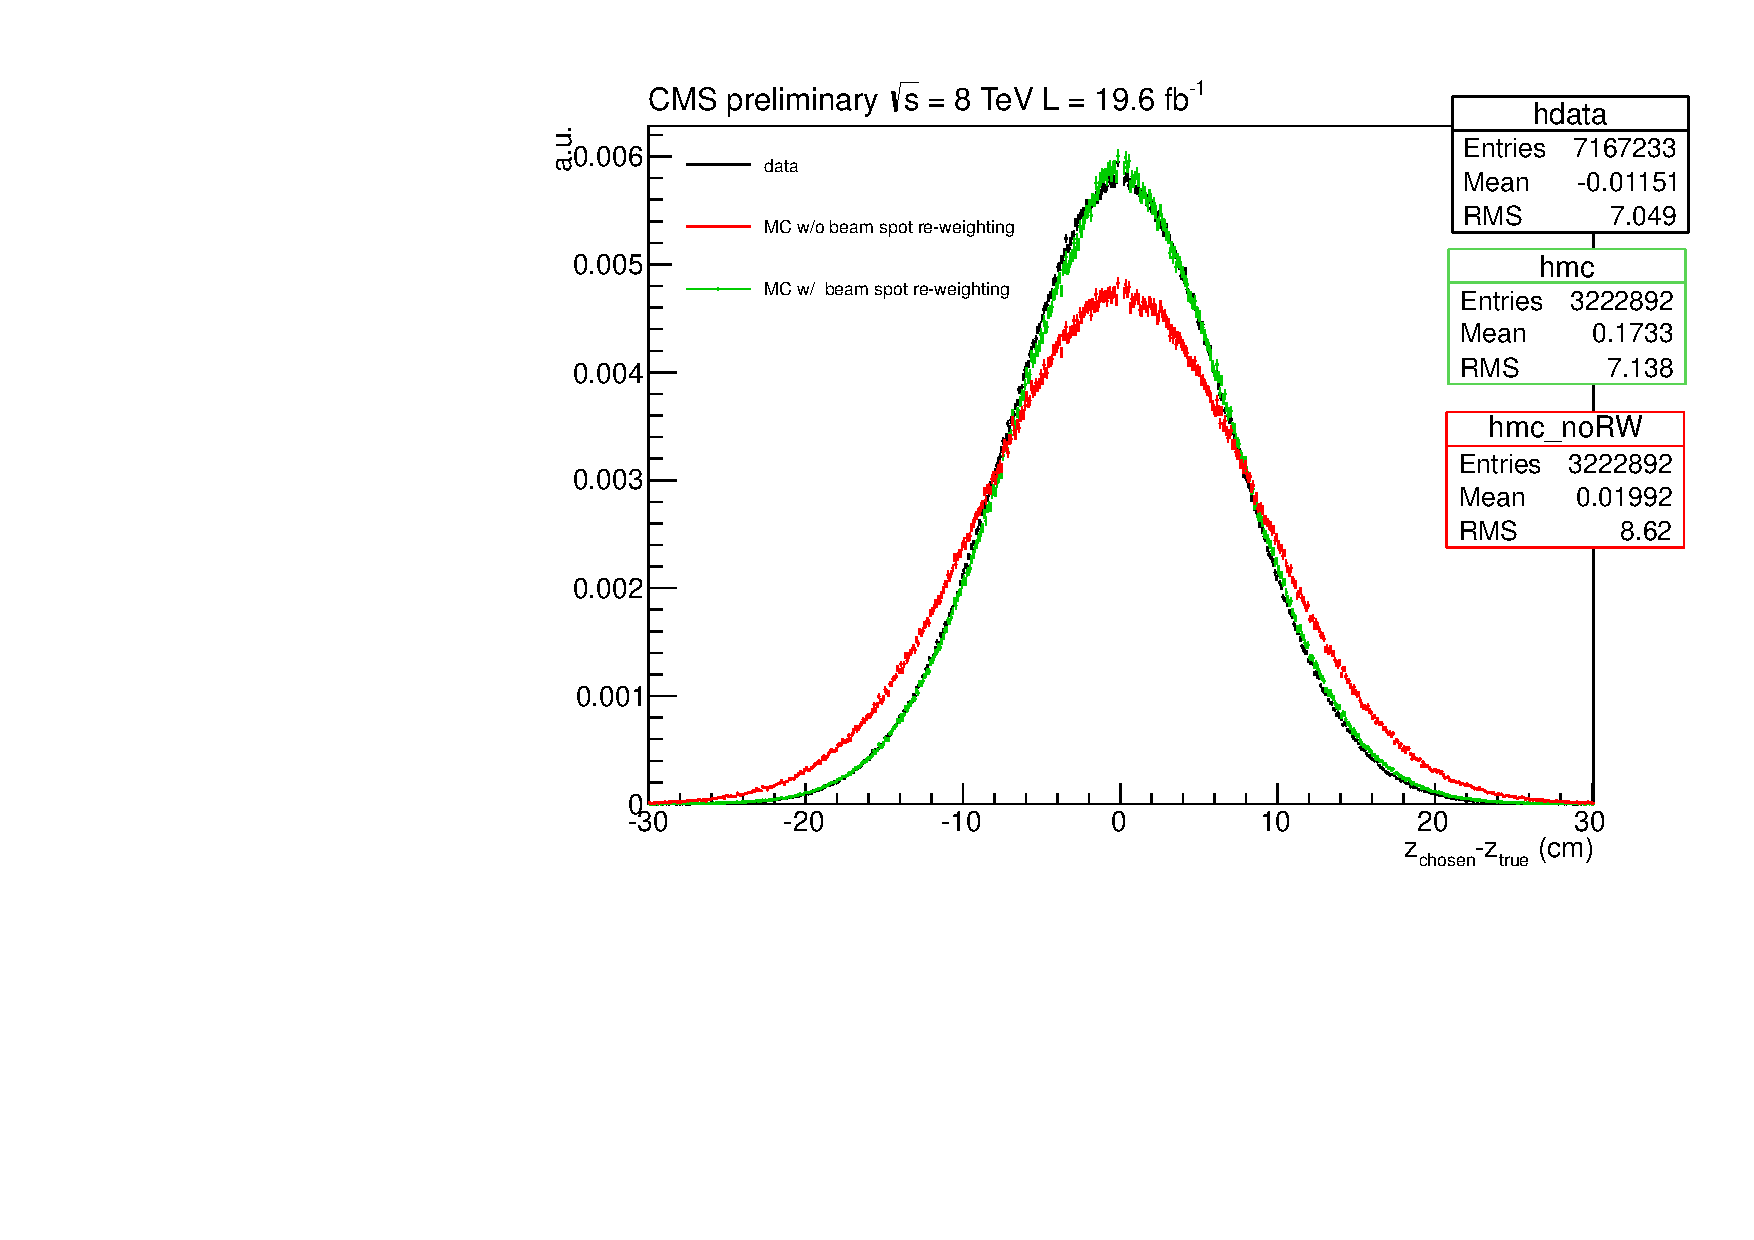
\includegraphics[width=0.55\textwidth]{ch3_comm_anal_comps/plots/beamspot.pdf}
  \caption{Distribution of $\Delta Z$ (the distance between the chosen vertex and the true vertex in the $z$ direction) for data (black), the \MC (red) and the \MC after beam spot reweighting (green) for \Zmumu events.}
  \label{fig:beamspot}
  \end{center}
\end{figure}

\section{Energy measurement of photons}
\label{sec:photon_energy}

The photon energy obtained from the supercluster sum described in Section~\ref{sec:ecal} even when including the intercalibration and transperency corrections shown in Figure~\ref{fig:ecal_laser_corrs} does not give the most optimal resolution for the energy measurement of photons at \CMS. On top of this energy (known as the \emph{raw} supercluster energy) it is also valuable to correct for additional energy losses. These arise from \emph{bremstrauhlung} where the photon converts in the material upstream of the \ECAL and the two electron legs radiate additional photons and thus the some of the photon shower is missed. Additional corrections should also account for local containment of the shower where some energy is lost through small gaps between \ECAL crystals and larger gaps between ``modules" or sections of crystals. These corrections are obtained using a specialised regression \BDT (see Sec.~\ref{sec:bdts}) trained on a \MC source of prompt photons from a sample containing photons and jets. The \BDT targets accurate measurements of individual photons' energy by correcting the raw supercluster energy and provides an estimate for the energy resolution of each photon given the position and shower shape of the supercluster. The training is done separately for barrel and endcap photons (as the cluster shapes look very different for these two distinct regions) and is also performed separately for the 7 and 8 TeV datasets. The following input variables are used:

\begin{itemize}
  \item The global position of the supercluster in \eta and \phi
  \item A collection of shower shape variables which aim at providing information on the likelihood and location of a photon conversion and the degree of showering in the material:
  \begin{itemize}
    \item The \rnine of the supercluster (as previously described in Section~\ref{sec:ecal})
    \item The ratio of the 5$\times$5 crystal energy to the raw supercluster energy (equivalent of $R_{25}$)
    \item The energy weighted \eta-width and \phi-width of the supercluster (in other words the spread of the shower)
    \item The number of basic clusters
    \item The ratio of energy in the \HCAL behind the supercluster to the \ECAL energy of the supercluster
    \item The ratio of the preshower energy to the raw supercluster energy (endcap only)
  \end{itemize}
  \item A collection of the seed crystal and the seed cluster variables which aim at providing information about energy lost through gaps and cracks between crystal and crystal modules:
  \begin{itemize}
    \item The relative energy and position of the seed cluster
    \item The local energy covariance matrix
    \item Energy ratios between the seed and the 3$\times$3 and 5$\times$5 areas around the seed
    \item The \eta and \phi index of the seed crystal and the relative position of the seed cluster to the crystal centre. 
  \end{itemize}
  \item Additionally the number of primary vertices and the median energy density, \rho, (see Sec.~\ref{sec:pileup}) are included to account for residual energy scale effects from pileup.
\end{itemize}

The regression is trained using an additional piece to that described in Section~\ref{sec:bdts} whereby the target is to predict the full probability distribution of the ratio of the true energy to the raw energy, $E_{true}/E_{raw}$. The target is a double crystal ball distribution which consists of a Gaussian core and power law tails on either side. This can be fully parametrised by six variables, the Gaussian mean and width ($\mu$, $\sigma$), the power parameters ($n_{L}$, $n_{R}$) and the power law tail cutoff parameters ($\alpha_{L}$, $\alpha_{R}$). Each of these parameters has a non-parametric dependence on the input variables, $\vec{x}$, and this is \emph{learned} by the regression training whilst simultaneously minimising the likelihood,

\begin{equation}
  -\ln \mathcal{L} = - \sum_{MC photons} \ln p(E_{true}/E_{raw} | \mu(\vec{x}),\sigma(\vec{x}),\alpha_{L}(\vec{x}),\alpha_{R}(\vec{x}),n_{L}(\vec{x}),n_{R}(\vec{x})),
\end{equation}

for the double crystal ball distribution, $p$. The most probable value for the true energy estimate of each photon is then given by,

\begin{equation}
  E(\vec{x},E_{raw}) = \mu(\vec{x})E_{raw}
\end{equation}

and the per-photon energy resolution is given by 

\begin{equation}
  \frac{\sigma_{E}(\vec{x},E_{raw})}{E(\vec{x},E_{raw})} = \frac{\sigma(\vec{x})}{\mu(\vec{x})}.
\end{equation}

In this way the regression predicts the full probability density of $E_{true}/E_{raw}$ and provides an estiamte of the optimal energy correction and the energy resolution per photon. A comparison of this distribution with a statistically independent \MC sample is shown for the 8~\TeV training in Figure~\ref{fig:regression_training}. The performance of the regression compared to the default photon reconstruction is shown in Figure~\ref{fig:regression_performance}.

\begin{figure}
  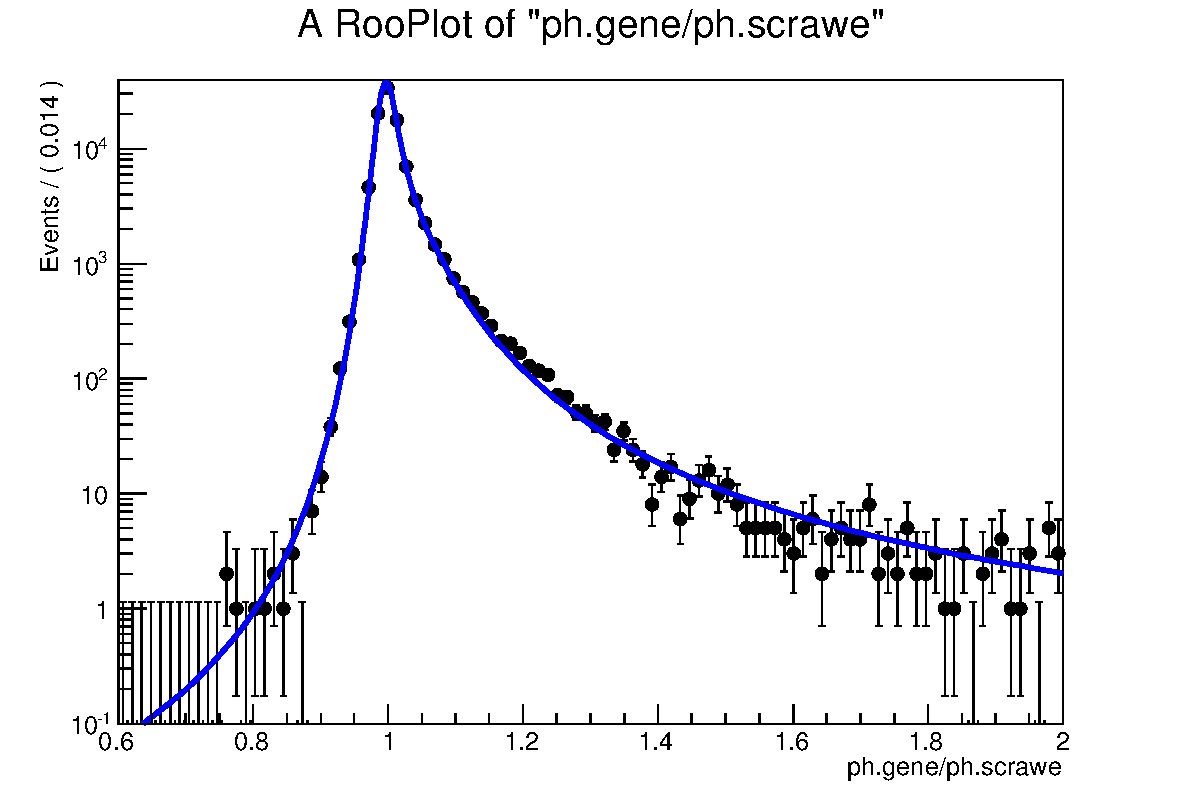
\includegraphics[width=0.48\textwidth]{ch3_comm_anal_comps/plots/regression_barrel.pdf}
  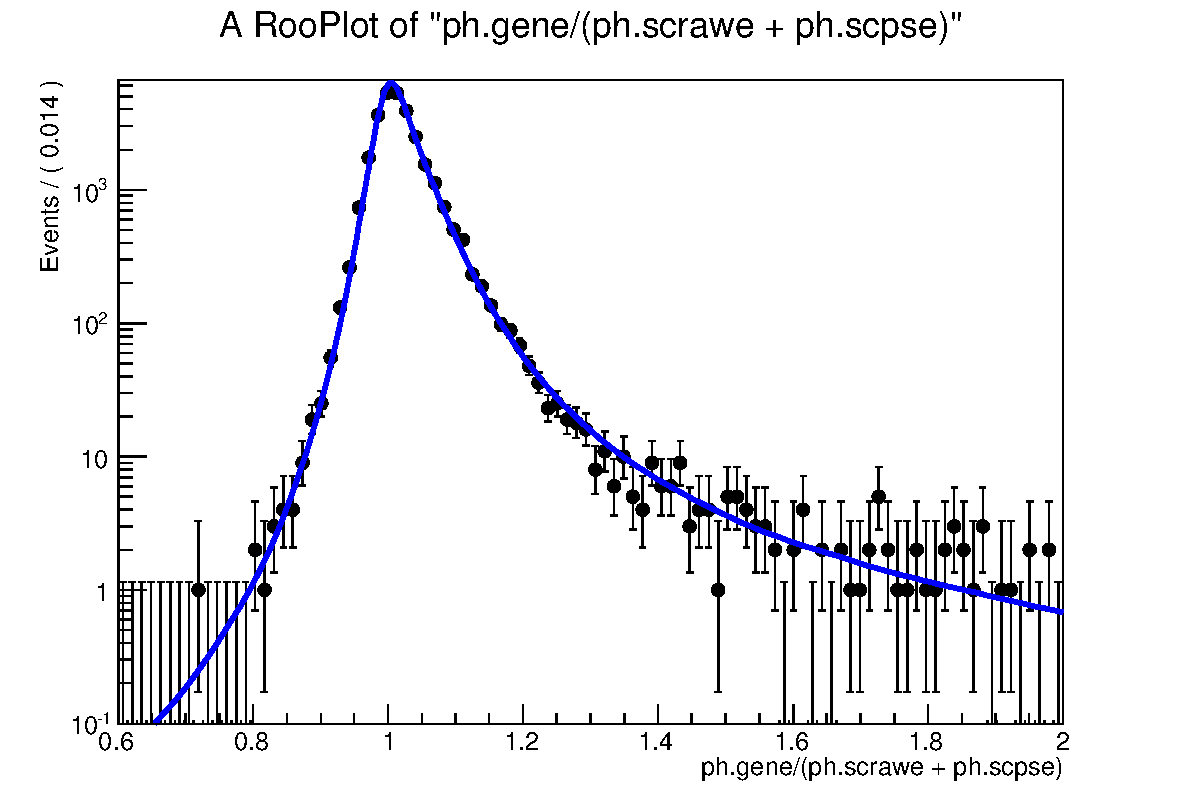
\includegraphics[width=0.48\textwidth]{ch3_comm_anal_comps/plots/regression_endcap.pdf}
  \caption{A comparison of the predicted probability density of $E_{true}/E_{raw}$ from the regression training (blue line) to the distribution in a statiscally independent \MC sample (black points) for barrel photons (left) and endcap photons (right). \red{PLOTS NEED TIDYING}}
  \label{fig:regression_training}
\end{figure}

\begin{figure}
  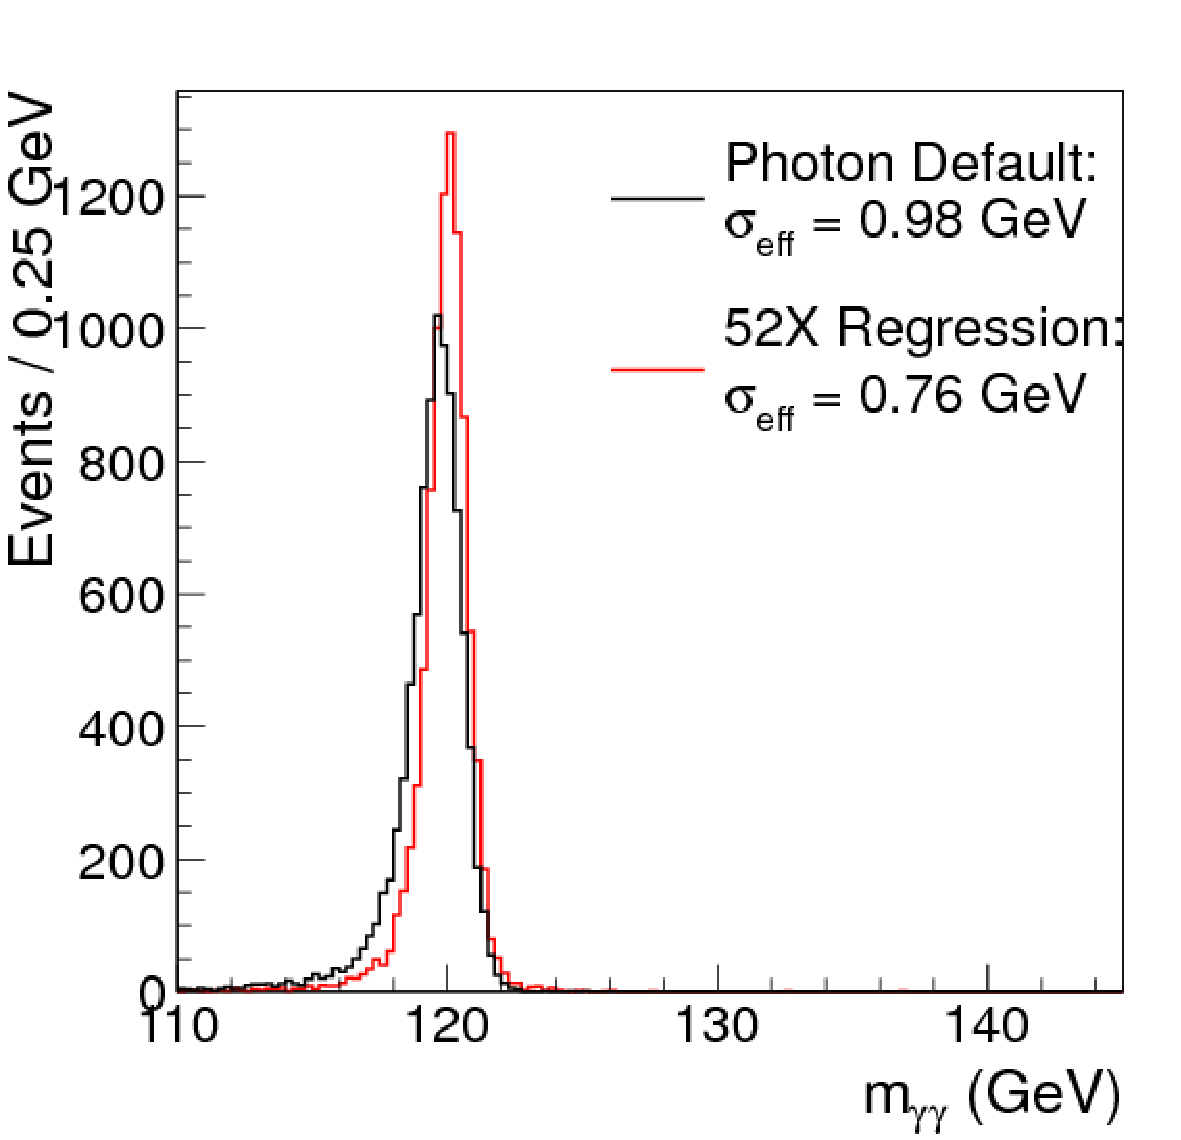
\includegraphics[width=0.24\textwidth]{ch3_comm_anal_comps/plots/regression_masscat0.pdf}
  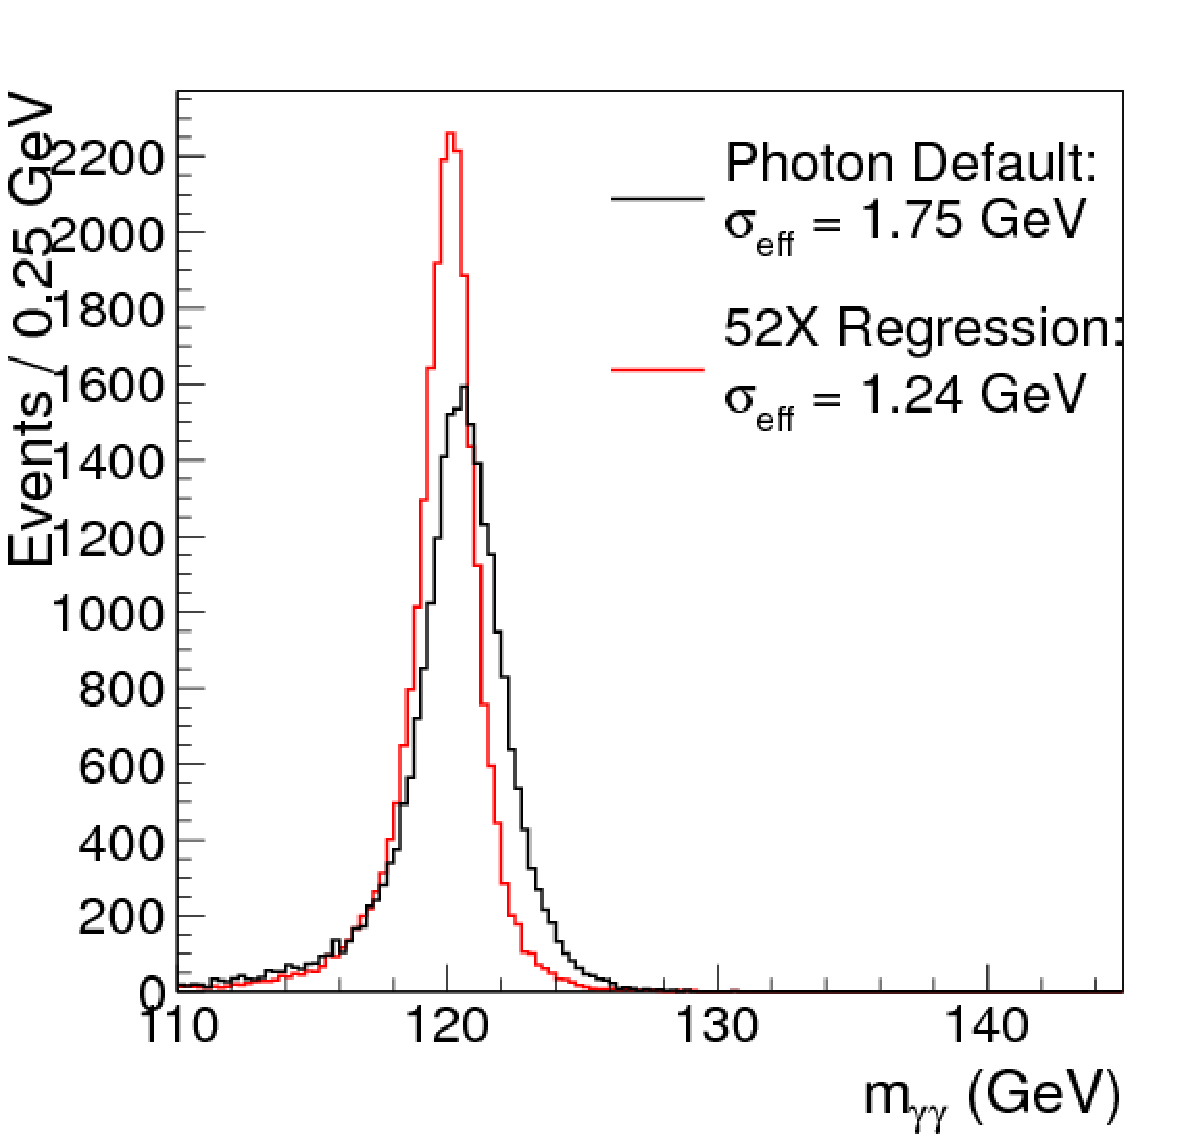
\includegraphics[width=0.24\textwidth]{ch3_comm_anal_comps/plots/regression_masscat1.pdf}
  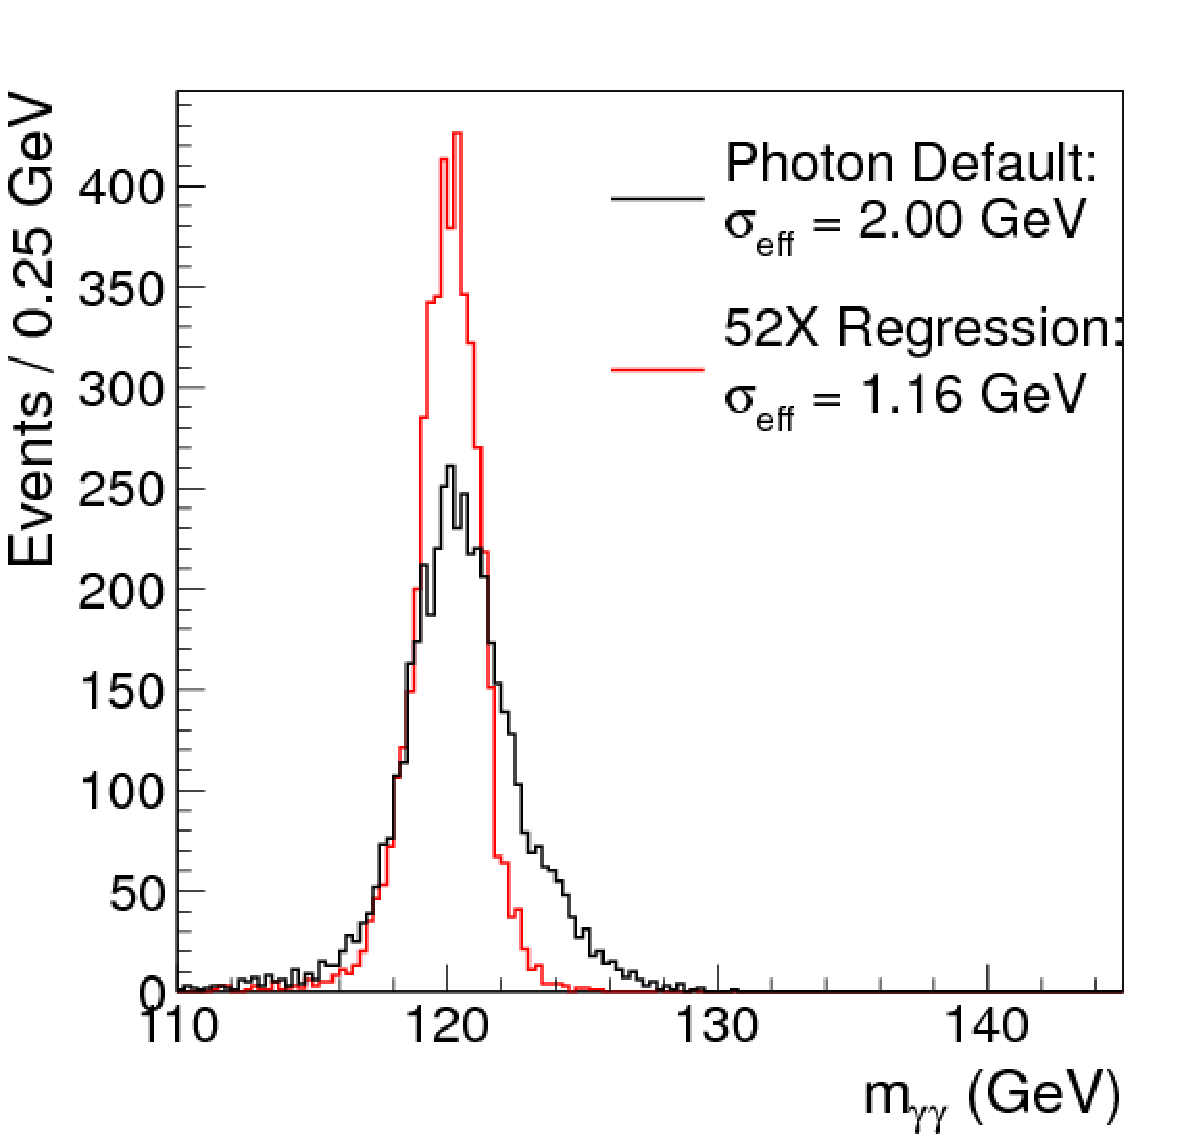
\includegraphics[width=0.24\textwidth]{ch3_comm_anal_comps/plots/regression_masscat2.pdf}
  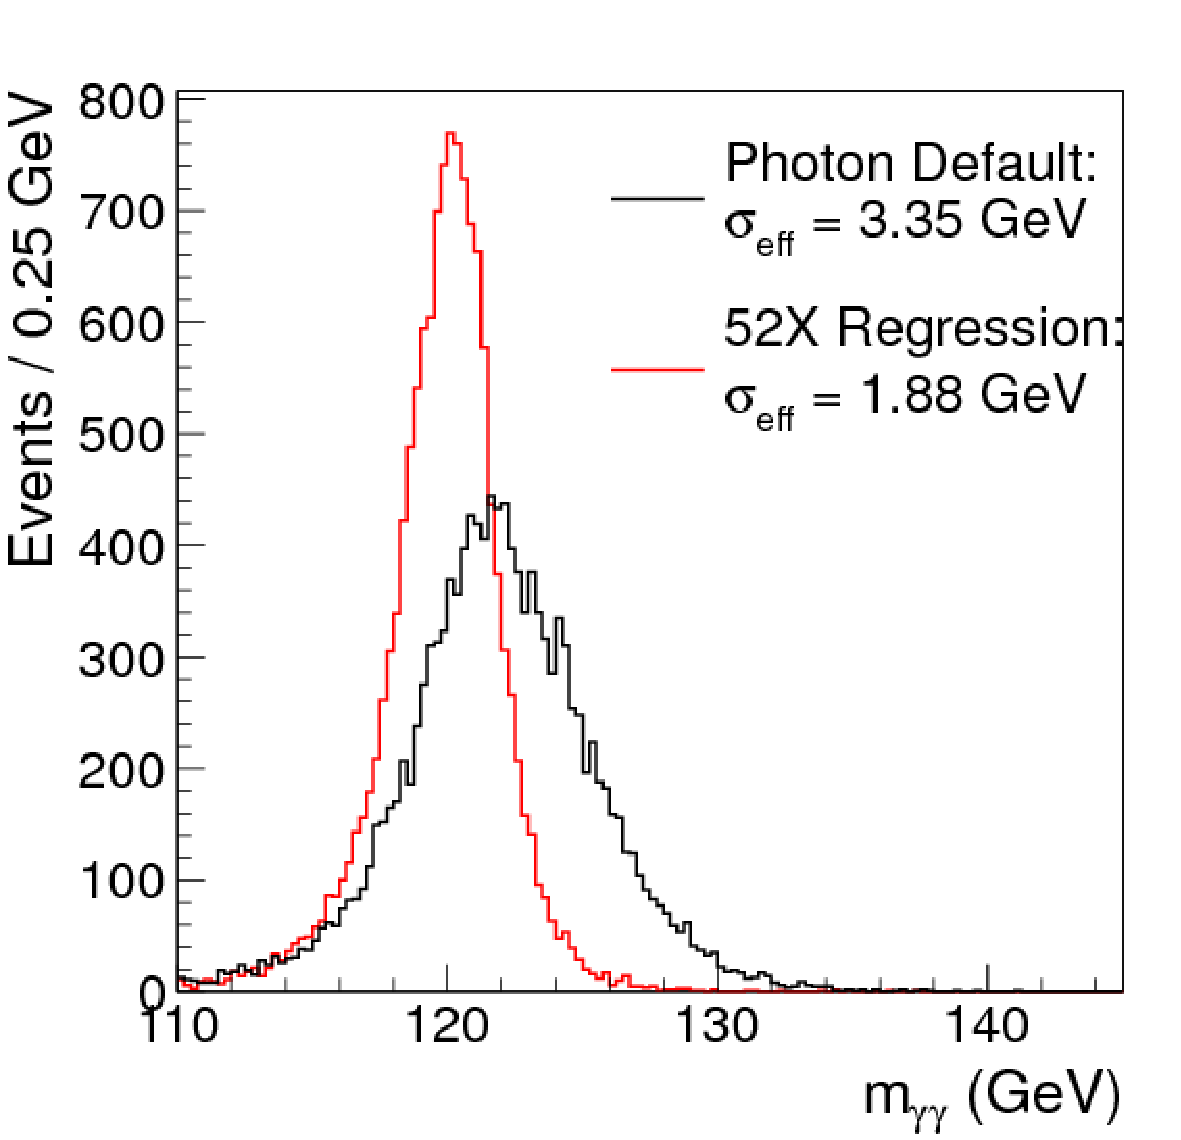
\includegraphics[width=0.24\textwidth]{ch3_comm_anal_comps/plots/regression_masscat3.pdf}
  \caption{A comparison of the regression performance compared to the photon default for the diphoton invariant mass on a \MC source of Higgs decays to two photons. This is shown when both photons are in the barrel (left two plots) when both photons have $\rnine>0.94$ (far left) and when at least one photon has $\rnine<0.94$ (middle left). When at least one photon is in the endcap (right two plots) when both photons have $\rnine>0.94$ (middle right) and when at least one photon has $\rnine<0.94$ (far right). The value shown in the legend of each is the effective width, $\sigma_{eff}$, which is defined as half of the narrowest interval which contains 68.3\% of the distribution. \red{PLOTS NEED TIDYING}.}
  \label{fig:regression_performance}
\end{figure}

\subsection{Correcting for residual discrepancies between data and Monte Carlo}

After application of the energy regression correction there are some remaining discrepancies between data and \MC. These residual effects are accounted for using \Zee events in data and simulation to correct the energy scale in the data and to apply an additional smearing term to the \MC with systematic uncertainties propagated through the analysis to account for the uncertainties on these corrections.

\subsubsection{Energy scale corrections to the data}

The supercluster energy is identical for electrons and photons so by correcting the supercluster energy scale to a known source, namely the mass of the $Z$-boson, in dielectron decays the smaller residual energy scale effects are accounted for. This can be done several times to account for various different effects. In the first stage scale corrections are derived in bins of time (run range) and \eta, after applying these corrections further, much smaller, residual effects are accounted for in bins of \rnine (the size of the effect is different for converted and non-converted photons). After applying both of these a further step is taken for the 8 TeV data in the barrel to derive residual corrections in bins of \ET. Consequently the total scale correction is a product of three corrections in 59 bins of time $\times$ 4 bins in \eta $\times$ 2 bins in \rnine $\times$ 6 bins in \ET (for the 8TeV barrel photons alone).

The strategy for deriving this corrections is to take \Zee events in data and \MC and extract the invariant dielectron mass in the relevant bin of interest. This mass distribution is fitted with a convolution of a Breit-Wigner (designed to handle the underlying Z line shape \refrqd) and a Crystal-Ball which models the calorimeter resolution effects and bremstrauhlung loses in the material upstream of the \ECAL. The Breit-Wigner parameters are fixed to the PDG values of $M_{Z}=91.188$~\GeV and $\Gamma_{Z}=2.495$~\GeV \refrqd whilst the Crystal-Ball parameters which model the detector effects are allowed to float. The scale correction, $\Delta E$, is then defined as the relative difference between the Crystal-Ball peak in data and simulation,

\begin{equation}
  \Delta E = \frac{m_{data}-m_{MC}}{m_{Z}}.
\end{equation}

\subsubsection{Energy resolution smearing the Monte-Carlo}

A similar method is used to extract a smearing factor that can be applied to the \MC such that the width of the invariant mass distribution in \Zee decays matches between data and \MC. This is done in 4 bins of \eta $\times$ 2 bins of \rnine and is parametrised as the quadratic sum of two resolution components: a constant term, $\Delta C$, and a stochastic term, $\Delta S$, which aims to model the expected resolution effects explained in Eq.~\ref{eq:energy_res} in Sec.~\ref{sec:ecal}. The smearing term, $\Delta\sigma$, is parametrised as,

\begin{equation}
  \Delta\sigma = \frac{\Delta S}{\sqrt{E_{T}}} \oplus \Delta C.
\end{equation}

The effect of the scale and smearing corrections is shown for the \Zee data and \MC samples in Figure~\ref{fig:scale_smearing_Zee} and for the analysis dataset after preselection with the electron veto inverted in Figures ~\ref{fig:scale_smearing_analysis_7TeV} and~\ref{fig:scale_smearing_analysis_8TeV}. Each of these corrections has an associated uncertainty and these uncertainties are propagated per photon through the analaysis. There are also additional uncertainties included which account for differences between electrons and photons and the difference between the $Z$ mass scale (around 90~\GeV) and the Higgs mass scale (around 125~\GeV). Systematic uncertainties are described in more detail in Section.~\ref{sec:systematics}.

\begin{figure}
  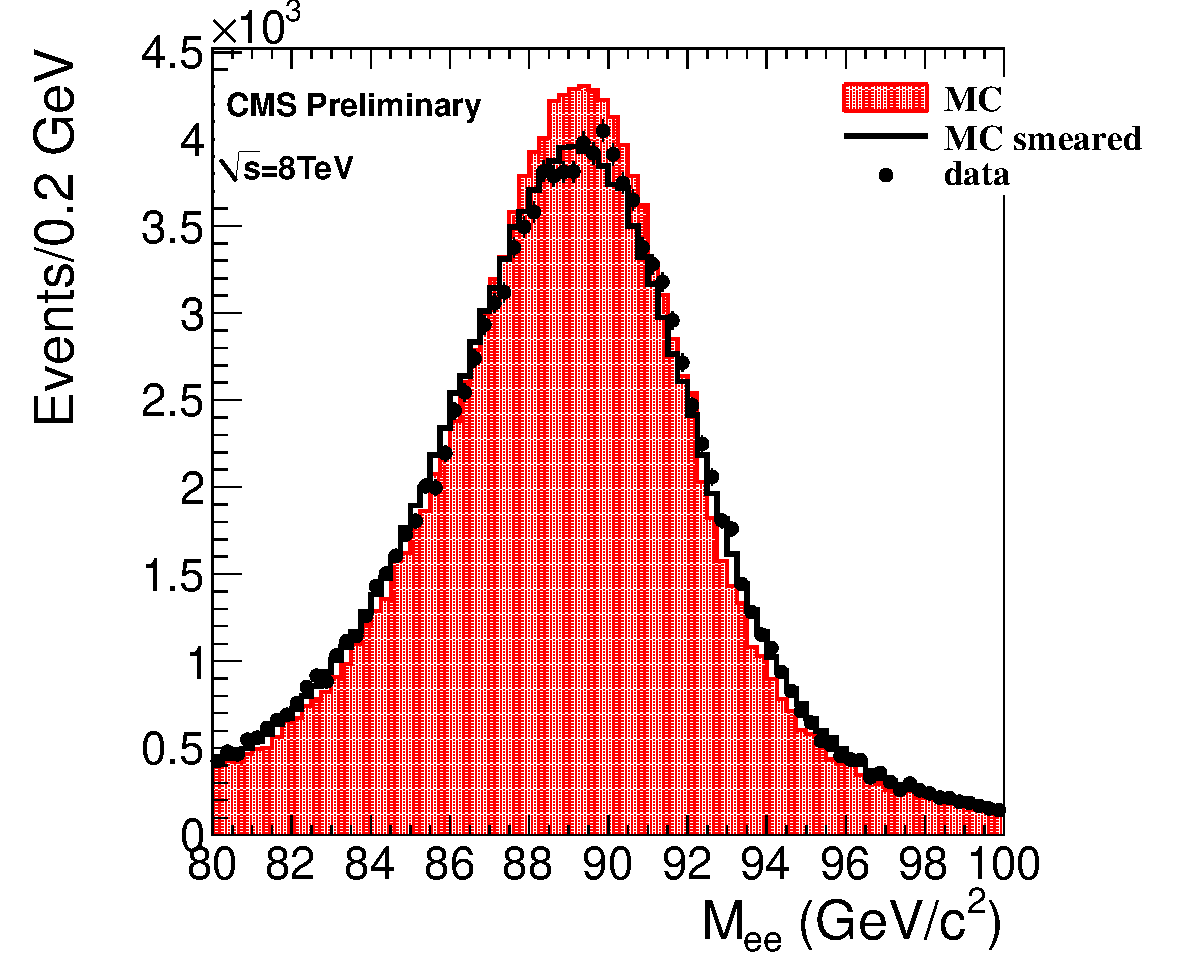
\includegraphics[width=0.48\textwidth]{ch3_comm_anal_comps/plots/smearing_EB_highEta_lowR9.pdf}
  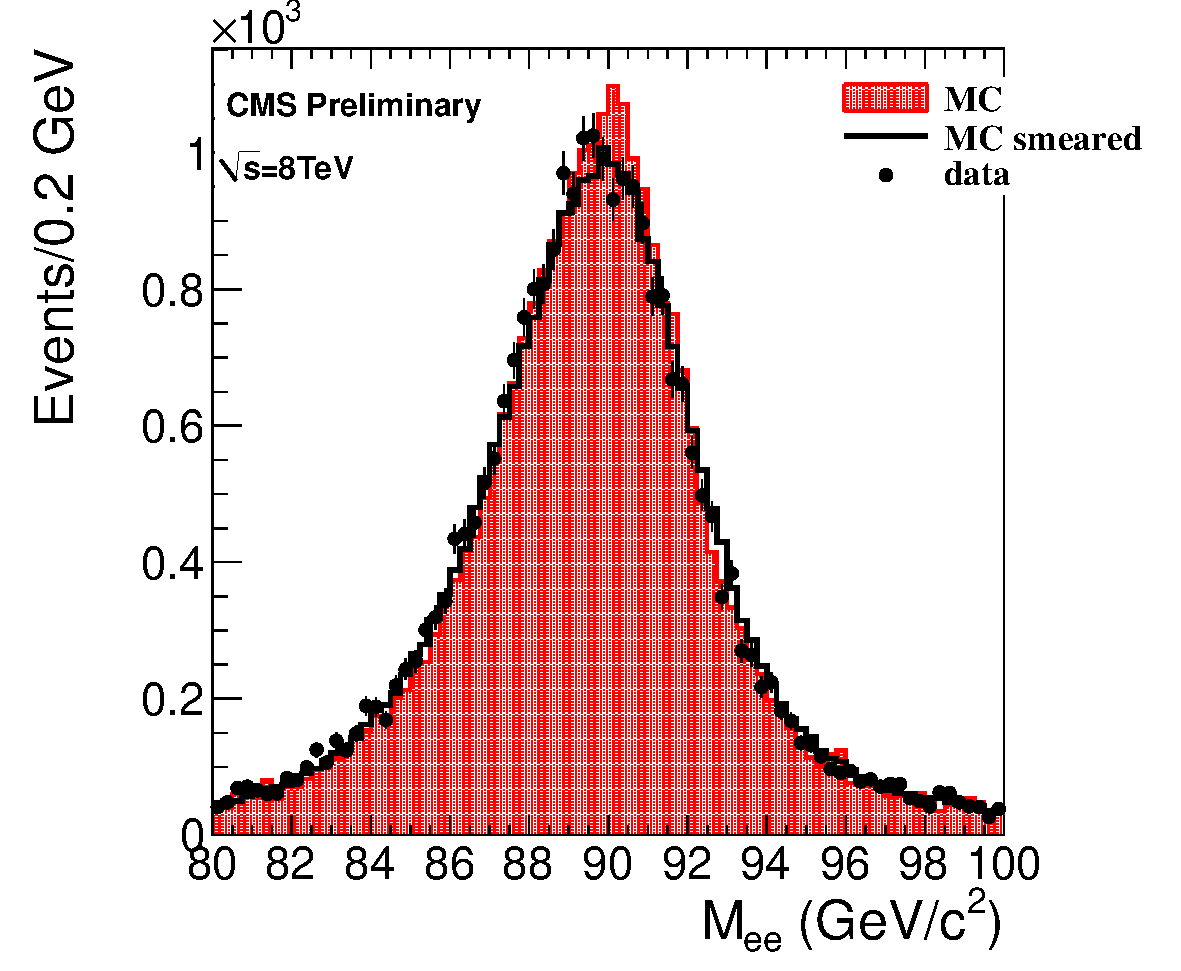
\includegraphics[width=0.48\textwidth]{ch3_comm_anal_comps/plots/smearing_EB_lowEta_highR9.pdf}
  \caption{The \Zee invariant mass shape comparison before and after the scale and smearing corrections are applied. Shown for 8~TeV for photons with $1.<|\eta|<1.444$ and $\rnine<0.94$ on the left and for photons with $|eta|<1.$ and $\rnine>0.4$ on the right.}
  \label{fig:scale_smearing_Zee}
\end{figure}

\begin{figure}
  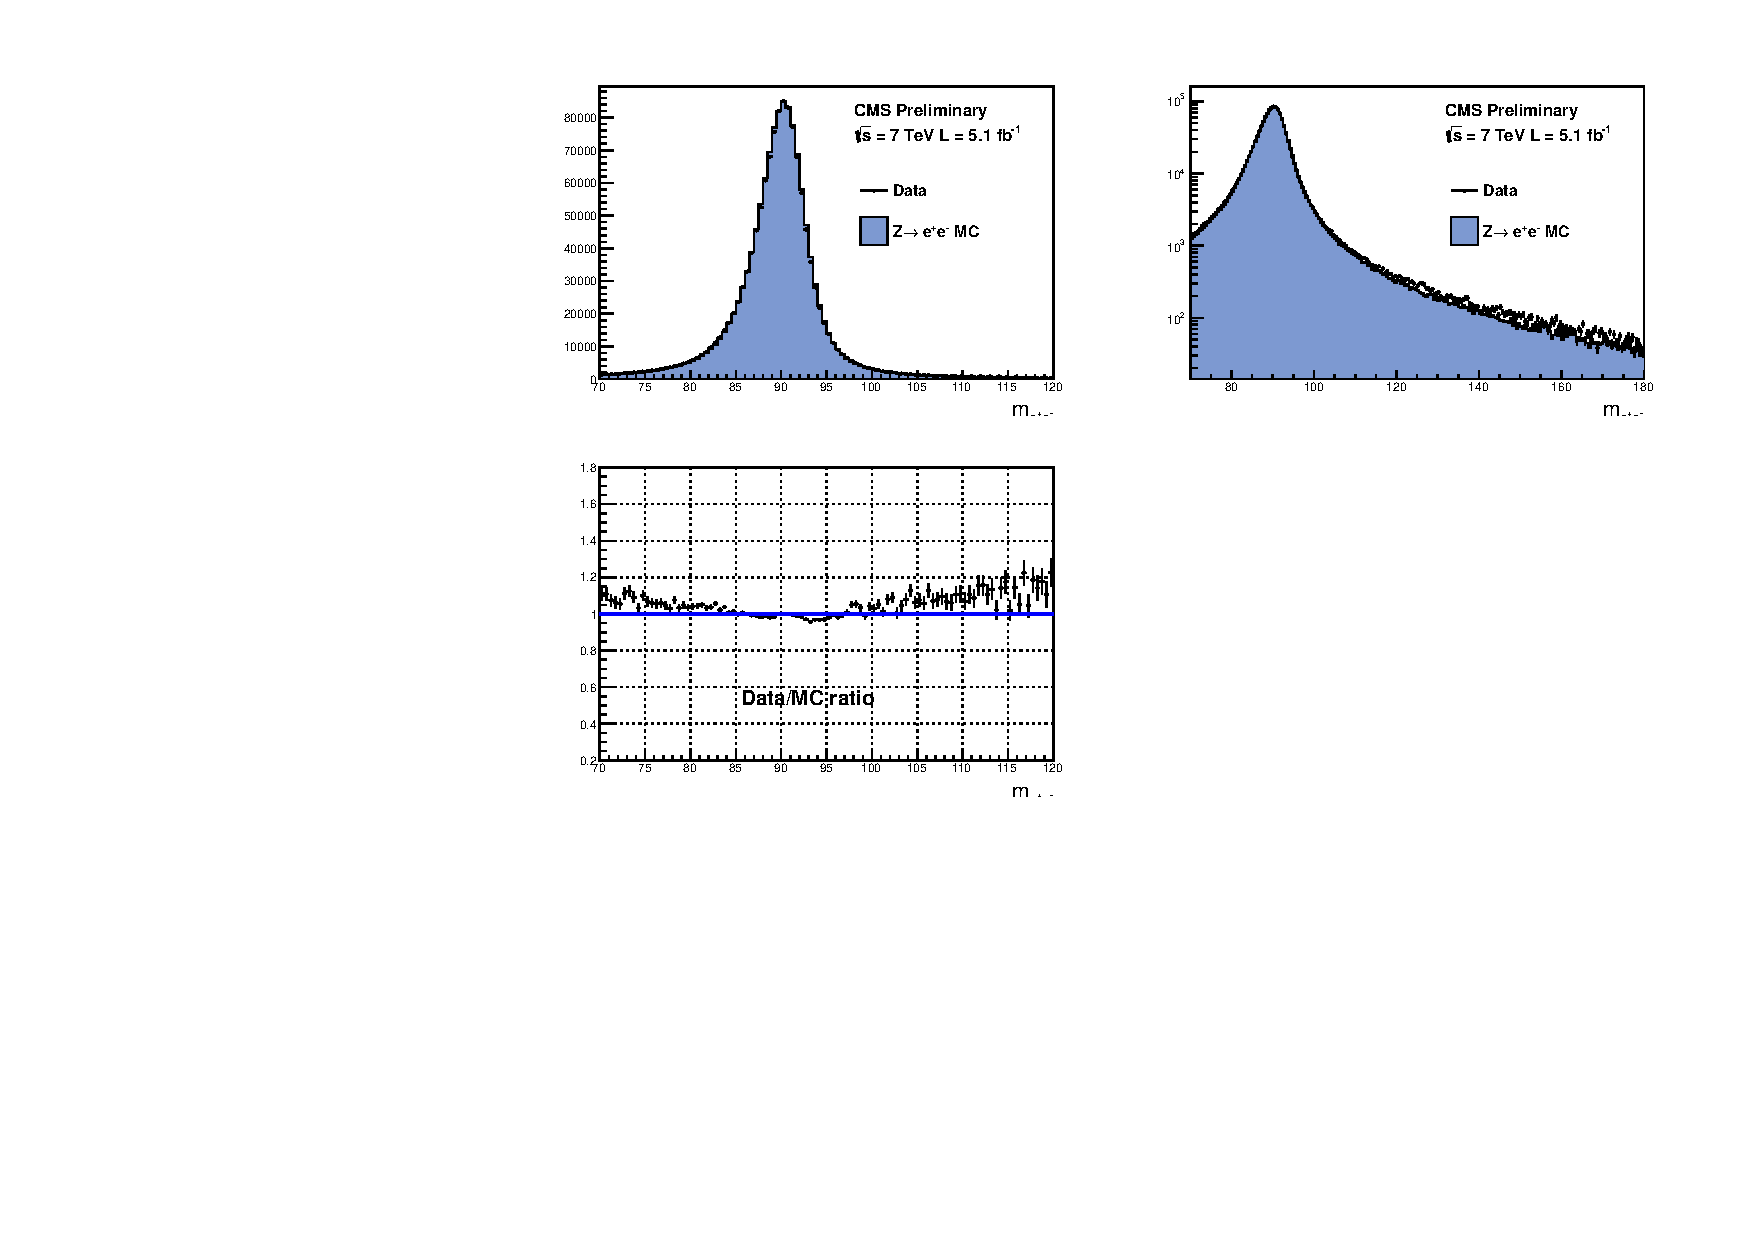
\includegraphics[width=0.9\textwidth]{ch3_comm_anal_comps/plots/smearing_mass_Zee_7TeV.pdf}
  \caption{The \Zee invariant mass distribution at 7TeV in data (black points) and \MC (blue histogram) for events which pass the analysis preselection in which the electron veto is inverted.}
  \label{fig:scale_smearing_analysis_7TeV}
\end{figure}

\begin{figure}
  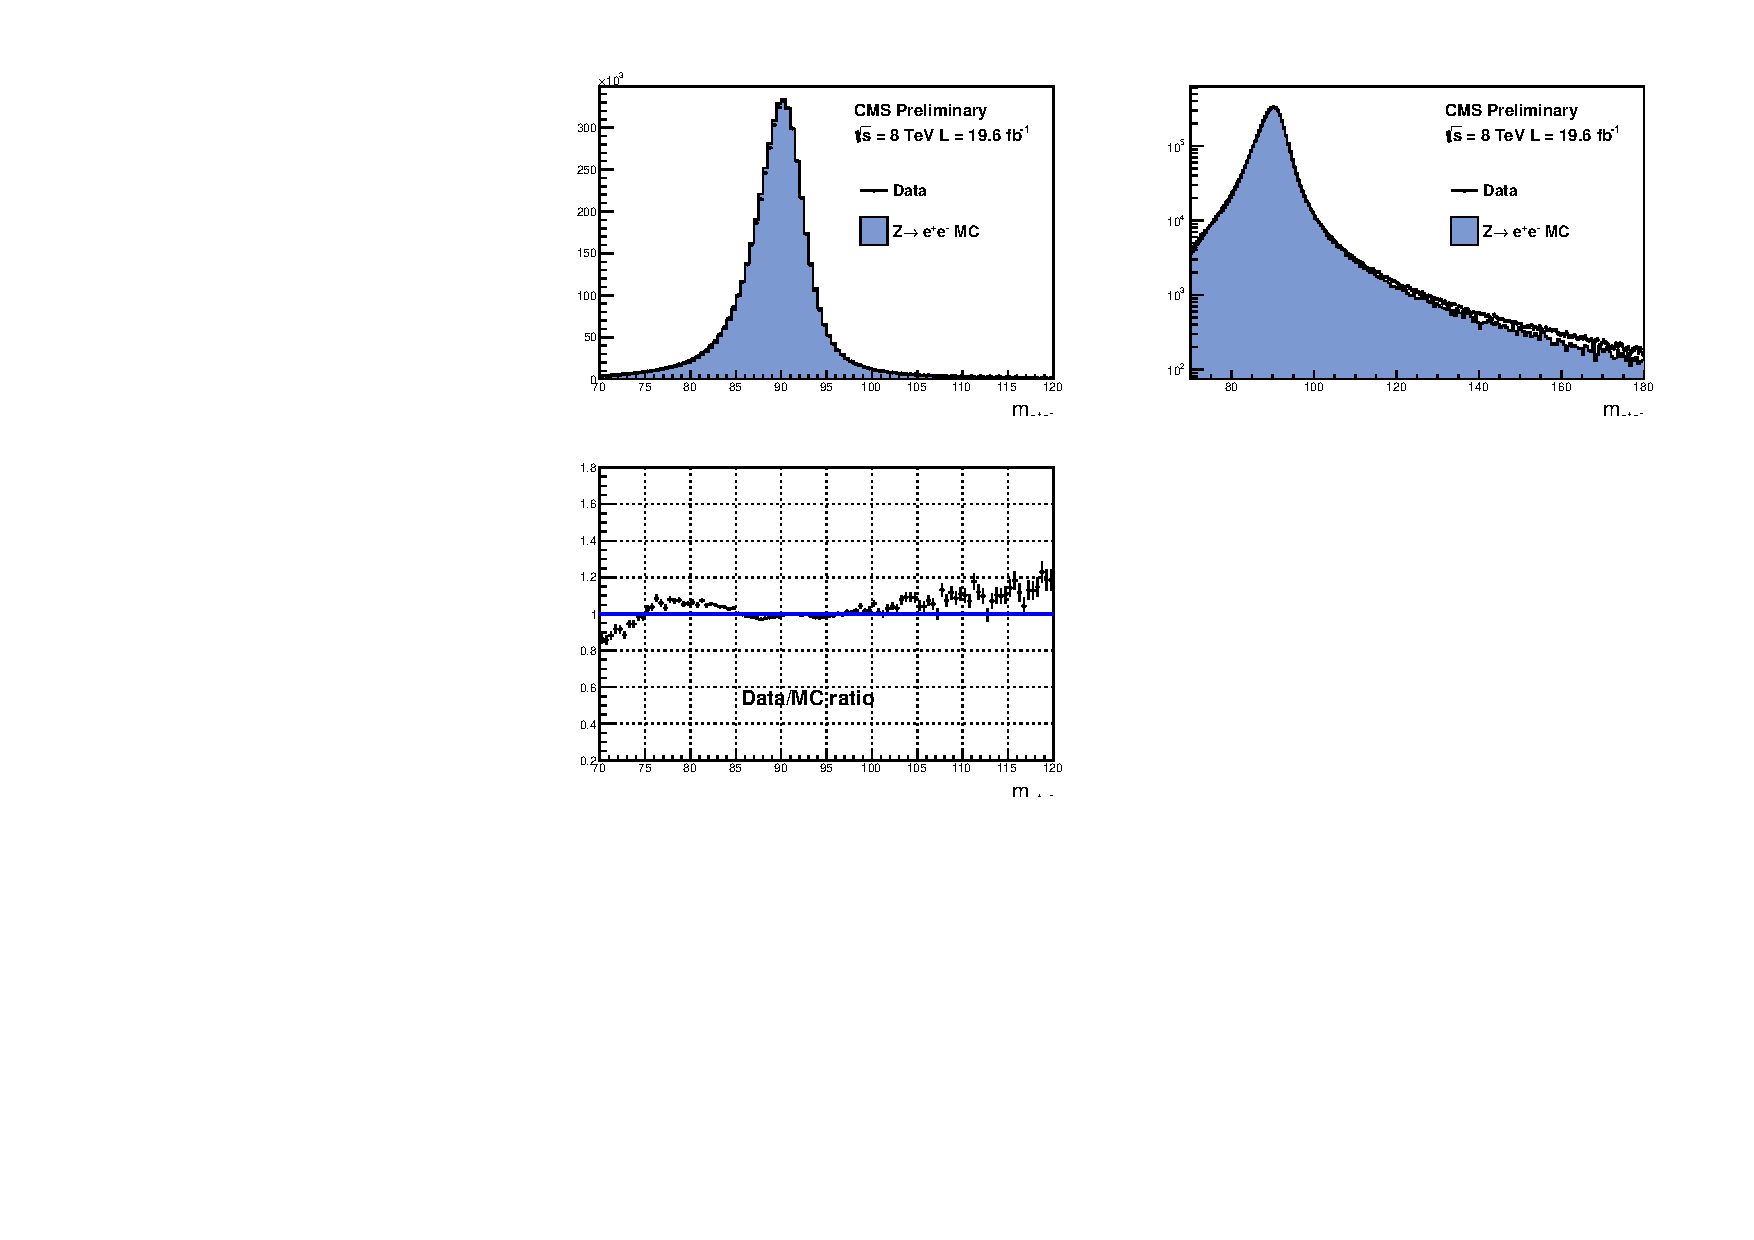
\includegraphics[width=0.9\textwidth]{ch3_comm_anal_comps/plots/smearing_mass_Zee_8TeV.pdf}
  \caption{The \Zee invariant mass distribution at 8TeV in data (black points) and \MC (blue histogram) for events which pass the analysis preselection in which the electron veto is inverted.}
  \label{fig:scale_smearing_analysis_8TeV}
\end{figure}

\section{Vertex reconstruction}
\label{sec:vtx_reco}

The resolution on the opening angle has a neglible effect if the correct vertex can be found within 10mm of the true interaction point. As seen in Sec.~\ref{sec:pileup_beamspot} the beamspot has an RMS spread of about 5~cm in the $z$ direction and there is an average of $\sim20$ vertices per bunch crossing. Because the beam direction is along the $z$-axis the spread of the vertex in the $x$ and $y$ directions is tiny (\red{number?}) and consequently mismeasurement of the primary vertex in the $x$-$y$ plane is small and has no impact on the mass resolution. By assigning the correct vertex to the diphoton pair, using other information in the tracking system, most of the mass resolution can be preserved. The method used to extract the primary vertex is a \BDT which exploits the correlation between the diphoton pair and the recoiling tracks from the underlying interaction as well as additional information in the tracking system from a photon conversion pair. The output of this per vertex \BDT is evaluated for each vertex in the event and the primary vertex is assigned as the one with the highest value (i.~e.~the value nearest 1.) of \BDT output. In addition, it is possible to construct another \BDT whose output is proportional to the probability that the chosen vertex is the correct one (described in Sec.~\ref{sec:bdt_prob}). This probability becomes a useful discrimnanting variable for the analyses later on.

The vertex \BDT uses the following input variables:

\begin{itemize}
  \item $\sum\limits_{i} |\vec{p}{}^{\;i}_{T}|^{2}$ - the sum of the transverse momentum squared of all of the tracks which originate from this vertex, representing how hard the interaction is at this vertex.
  \item $\sum\limits_{i} \bigl(\vec{p}^{\;i}_{T} \cdot \frac{\vec{p}^{\gamma\gamma}_{T}}{|\vec{p}^{\gamma\gamma}_{T}|}\bigr)$ - the sum of the magnitude of the transverse momentum of each track orginating from this vertex relative to the transverse momentum of the diphoton system, representing the recoil of the tracks to the diphoton system.
  \item $\bigr(|\sum\limits_{i} \vec{p}^{\;i}_{T}| - \vec{p}^{\gamma\gamma}_{T}\bigl) / \bigr(|\sum\limits_{i} \vec{p}{}^{\;i}_{T}| + \vec{p}^{\gamma\gamma}_{T}\bigl)$ - the asymmetry between diphoton system and the other tracks originating from this vertex.
  \item $|z_{v}-z_{c}|/\sigma_{c}$ - this is added for events which contain at least one photon conversion where $z_{v}$ is the $z$ position of the vertex in question and $z_{c}$ and $\sigma_{c}$ are the estimated $z$ position of the vertex from conversion information and its approximate error as defined below.
\end{itemize}

For events which contain at least one photon conversion, the conversion tracks and/or the conversion momentum can be used to point back to the beam line and estimate the vertex position. This can be acheived in one of two ways. In cases where the conversion occurs early, i.~e.~in one of the first layers of the tracking system, then the two electron legs of the conversion will leave two clean and distinct tracks. This means that the momentum of the conversion pair can be accurately reconstructed and used to point from the conversion vertex position back to the beam line and thus the nearest primary vertex. In cases where the conversion occurs late in the tracking system there are not enough track hits to accurately reconstruct the momentum of the conversion pair, however the incident position of the photon at the \ECAL face is well known in this case, so the line which connects the \ECAL position with the conversion vertex can be used to point back to the beam line. This is diagramtically represented in Figure~\ref{fig:conv_diags} for both cases.

\begin{figure}
  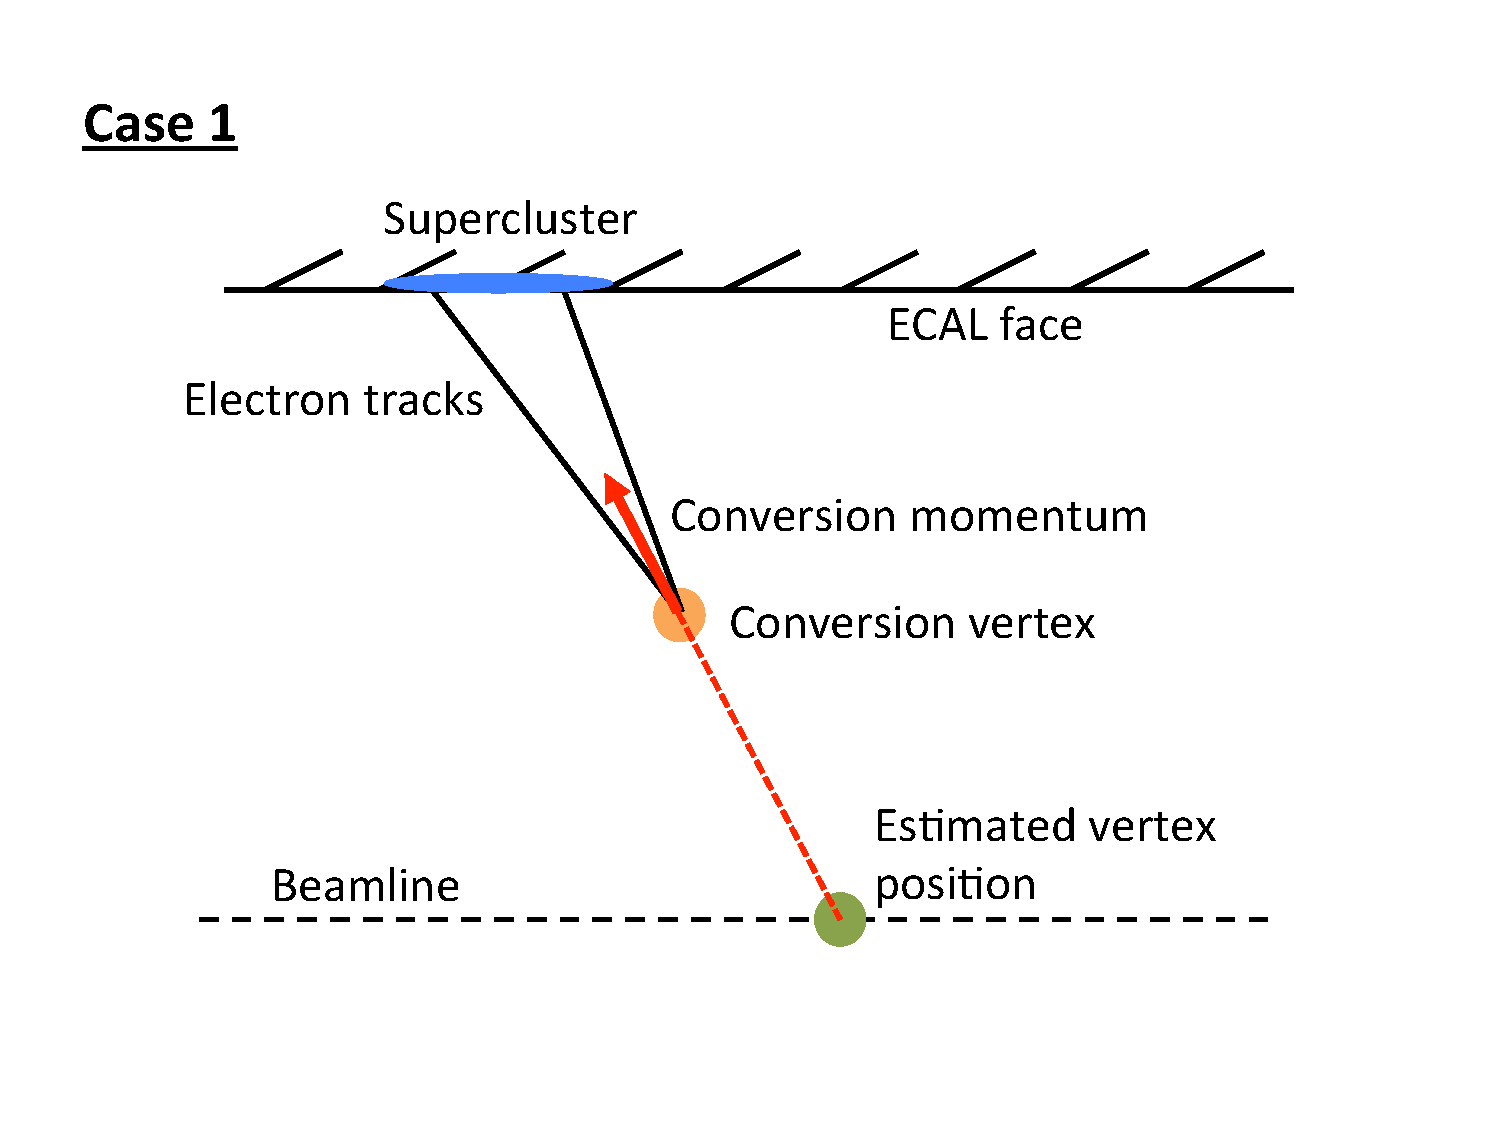
\includegraphics[width=0.49\textwidth]{ch3_comm_anal_comps/plots/ConversionDiagCase1.pdf}
  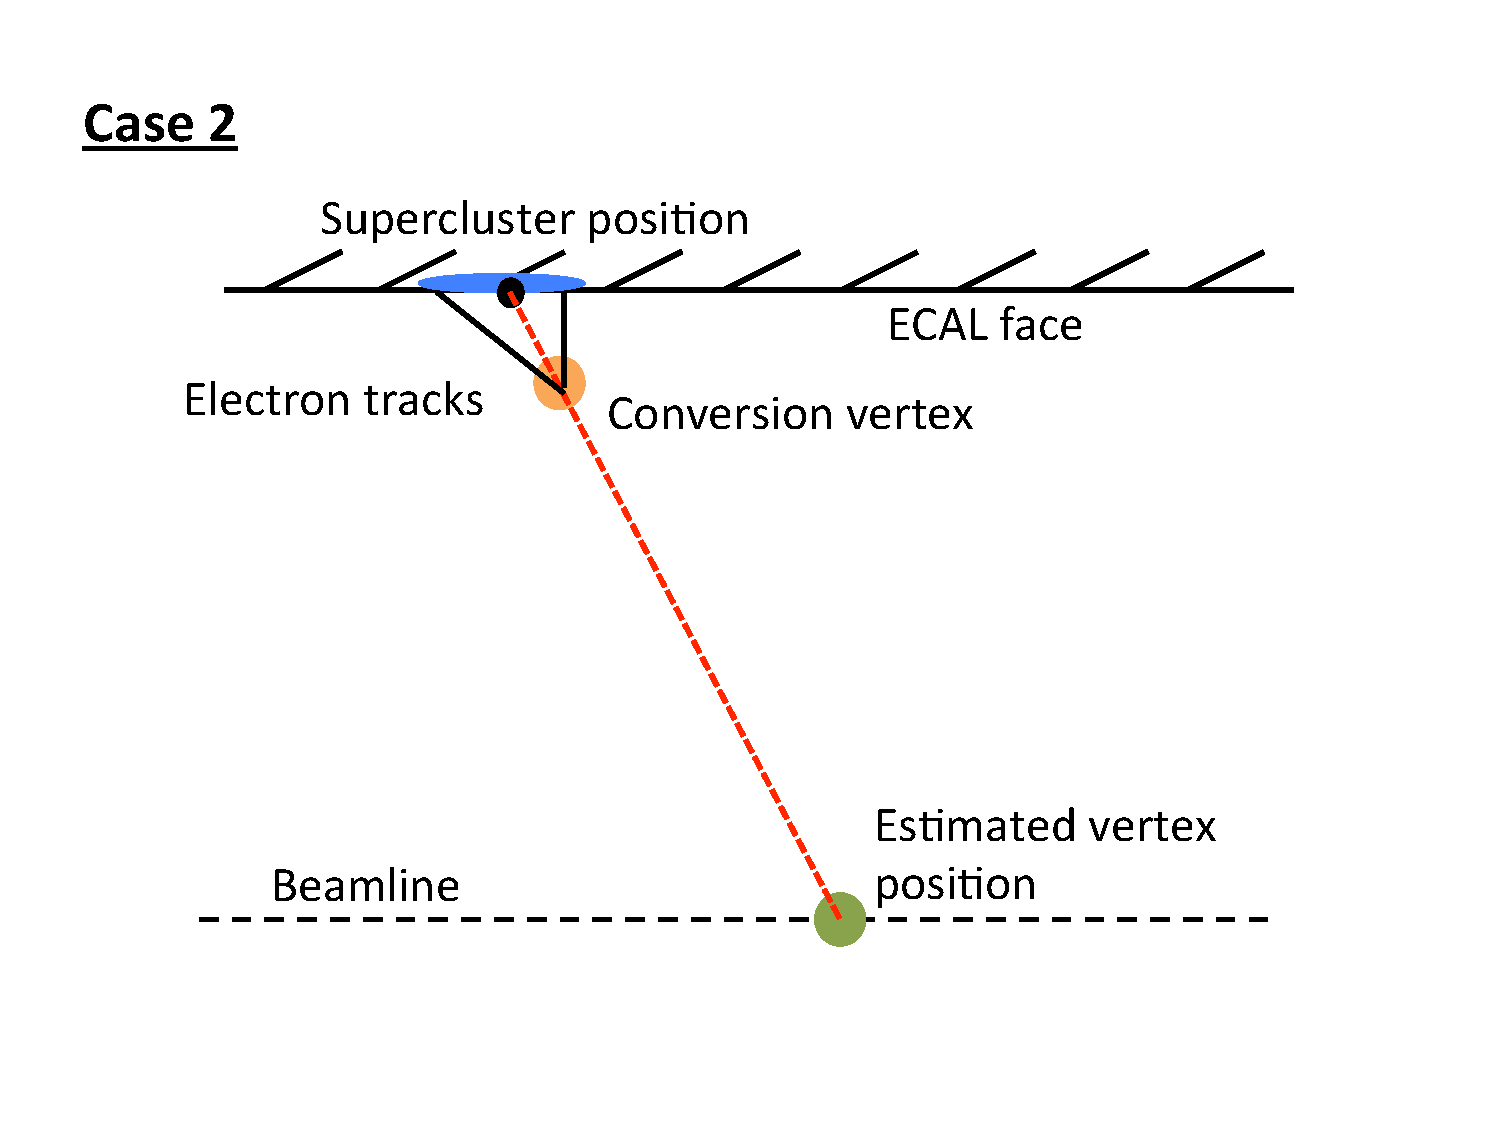
\includegraphics[width=0.49\textwidth]{ch3_comm_anal_comps/plots/ConversionDiagCase2.pdf}
  \caption{A representation of the two methods for locating the primary vertex using photon conversion information. The left plot is for cases where the conversion occurs early enough in the tracker that the two electron tracks can be used to construct the converted pair momentum which is combined with the conversion vertex position to point back to the beam line. The right plot is for cases where the conversion occurs late in the tracker and the energy weighted supercluster position and the conversion vertex position are used to point back to the beam line.}
  \label{fig:conv_diags}
\end{figure}

For Case 1 conversions the primary vertex $z$ position is calculated as,

\begin{equation}
  z_{PV} = z_{conv} - r_{conv}\cot(\alpha),
\end{equation}
where $z_{conv}$ is the z position of the conversion vertex, $r_{conv}$ is the distance of the conversion vertex from the beam line and $\alpha$ is the angle between the beam line and the conversion momentum.

For Case 2 conversions the primary vertex $z$ position is calculated as,

\begin{equation}
  z_{PV} = \frac{z_{conv}-r_{conv}}{(r_{SC}-r_{conv})(z_{SC}-z_{conv})},
\end{equation}
where $z_{conv}$ and $z_{SC}$ are the $z$ positions of the conversion vertex and supercluster respectively, and $r_{conv}$ and $r_{SC}$ are the distance of the conversion vertex and the supercluster from the beamline.

There are 6 regions of the tracking system (refer back to Figure~\ref{fig:cms_tracker}). When the conversion vertex is located in one of the inner regions; Pixel Barrel, Pixel Forward, TID, the Case 1 
conversion information is included in the \BDT, otherwise the Case 2 conversion information is used. The resolution on the primary vertex position in conversions is estimated per tracking region by calulating the effective width \footnote{Half the narrowest interval which contains 68.3\% of the distribution} of the distribution of the difference between the $z$ position of the primary vertex without conversion information and the $z$ position of the primary vertex using conversion information alone, $\Delta z=z_{PV}-z_{conv}$. Consequently the fourth input variable to the \BDT, shown in the list above as $|z_{v}-z_{c}|/\sigma_{c}$, is effectively a pull distribution for the conversion vertex. The \BDT will favour vertices whose value of this variable is near zero.

The \BDT is trained on a sample of \Hgg \MC events. It is tested with a statistically independent sample and further validated using \Zmumu decays in data and \MC. The efficiency is measured in data using the \Zmumu channel where the muon tracks are removed from the \BDT variables to simulate a diphoton like situation in data. The distributions of the input variables are shown for the \Hgg training sample in Figure~\ref{fig:vertex_bdt_inputs}. The \BDT response is shown for \Zmumu data and \MC for both the signal (right vertex) and background (wrong vertex) in Figure~\ref{fig:vertex_bdt_response}. The chosen primary vertex is the one which gives the highest score \BDT output. The effiency of the vertex selection as a function of the $Z$ \pT and the number of reconstructed vertices as measured in \Zmumu data and \MC samples is shown in Figure~\ref{fig:vertex_bdt_efficiency}. 

\begin{figure}
  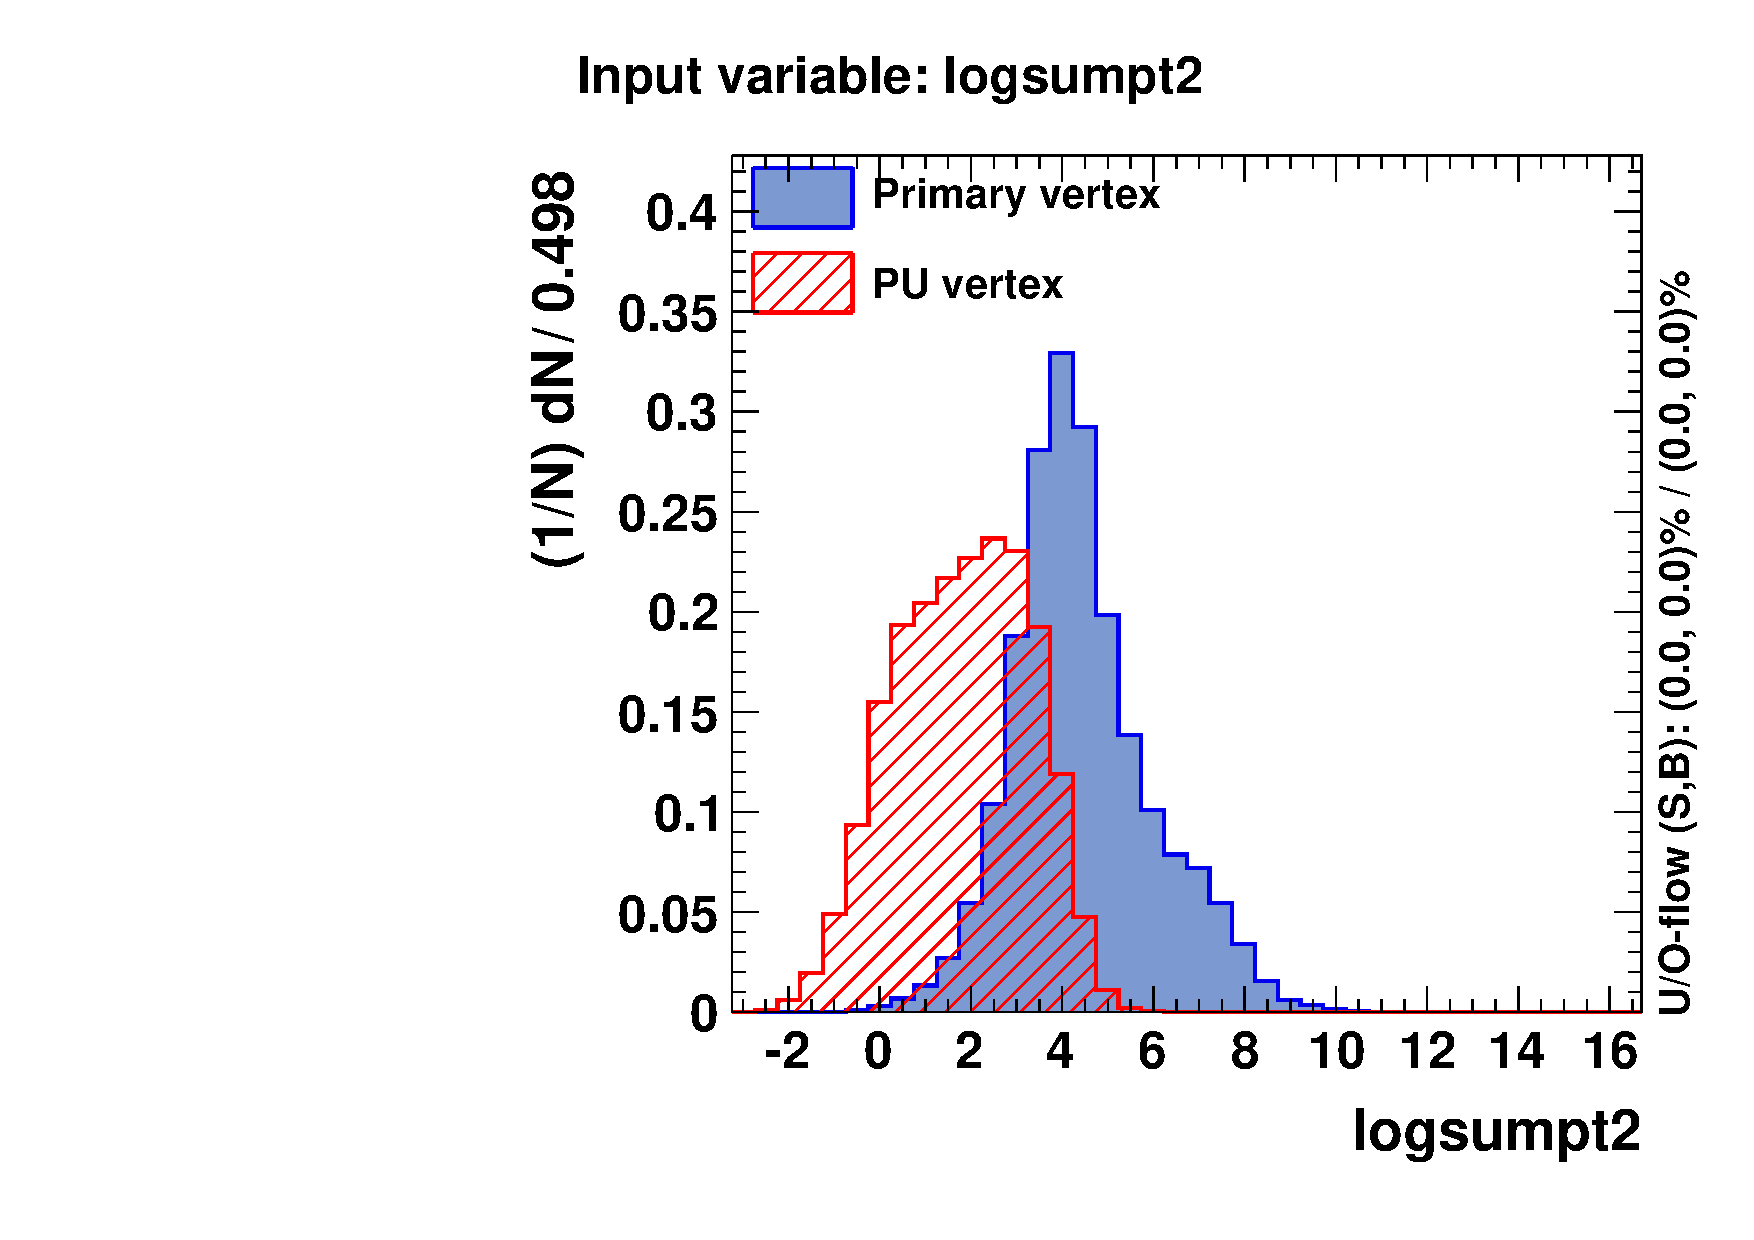
\includegraphics[width=0.48\textwidth]{ch3_comm_anal_comps/plots/vertex_bdt_input0.pdf}
  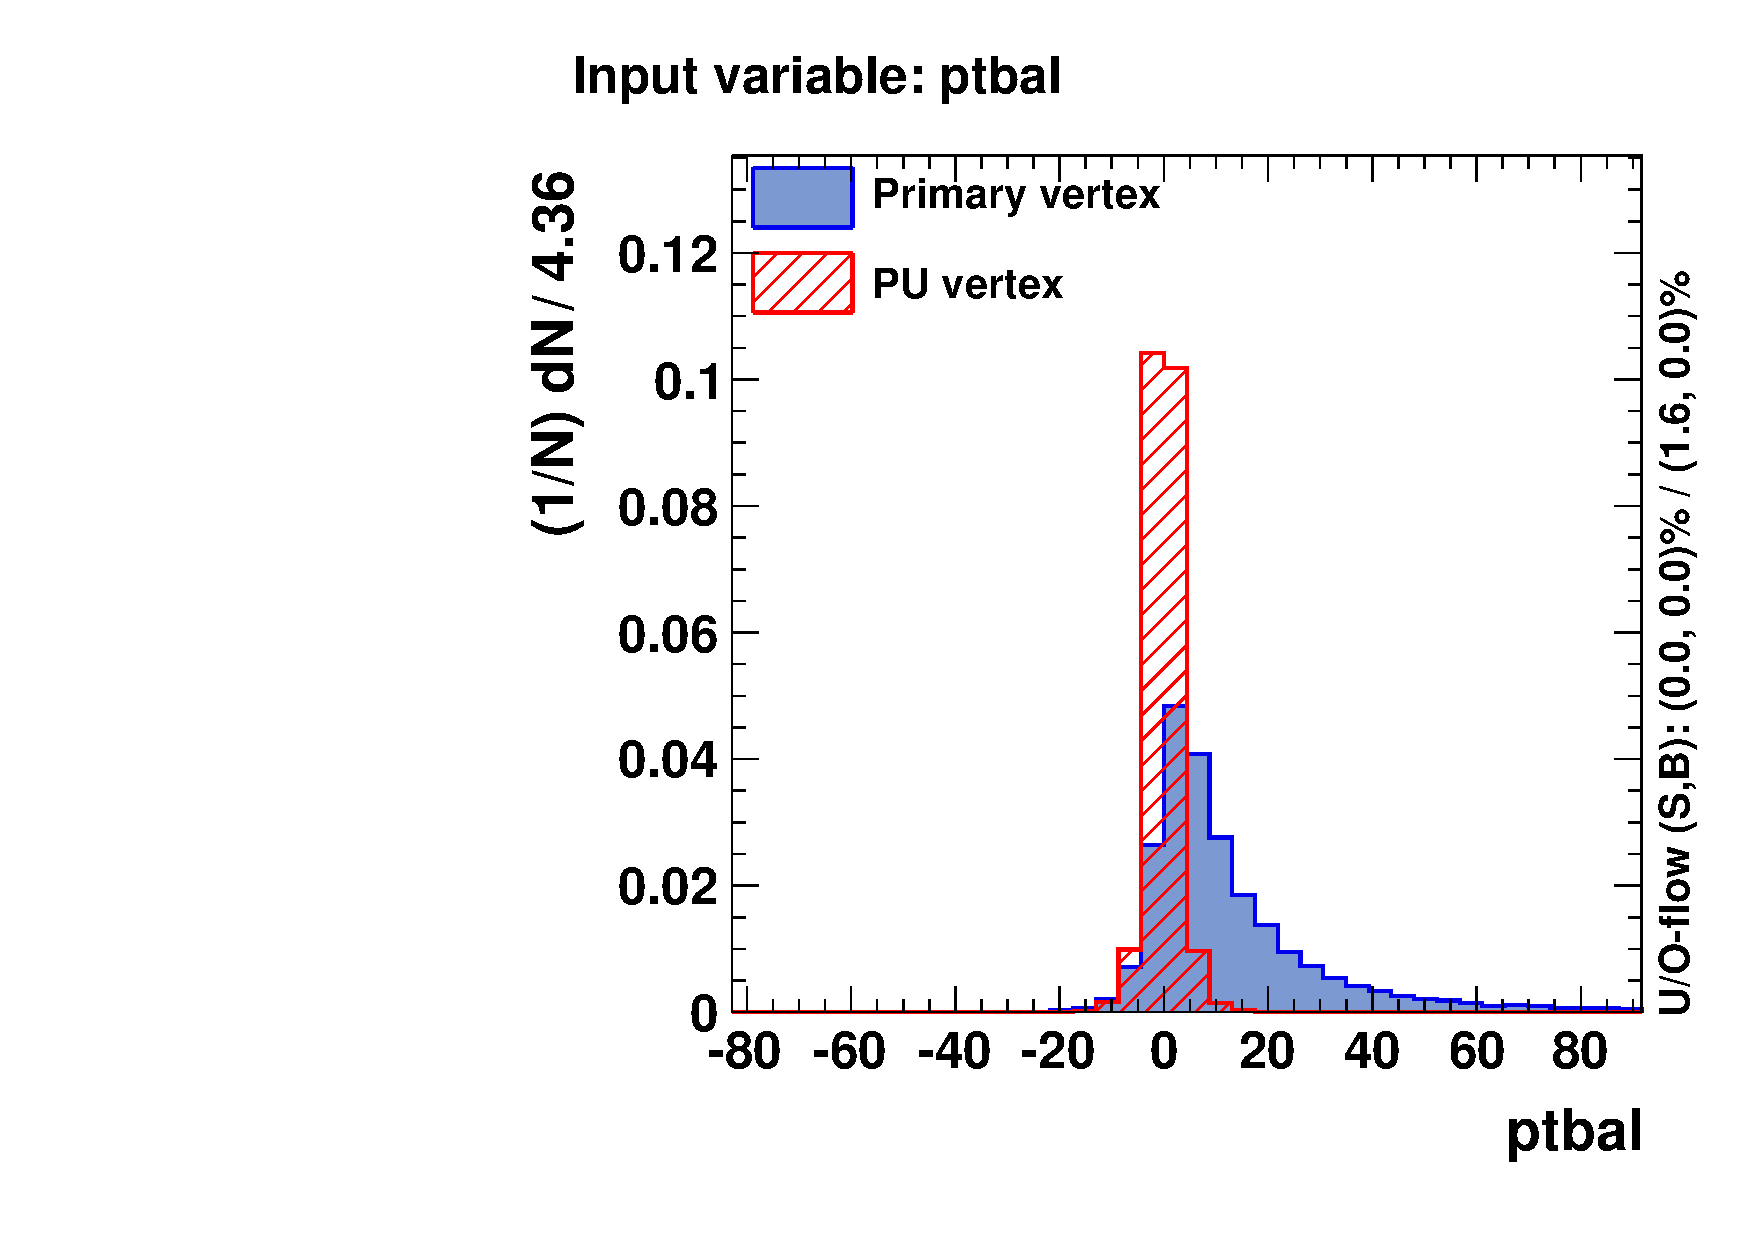
\includegraphics[width=0.48\textwidth]{ch3_comm_anal_comps/plots/vertex_bdt_input1.pdf} \\
  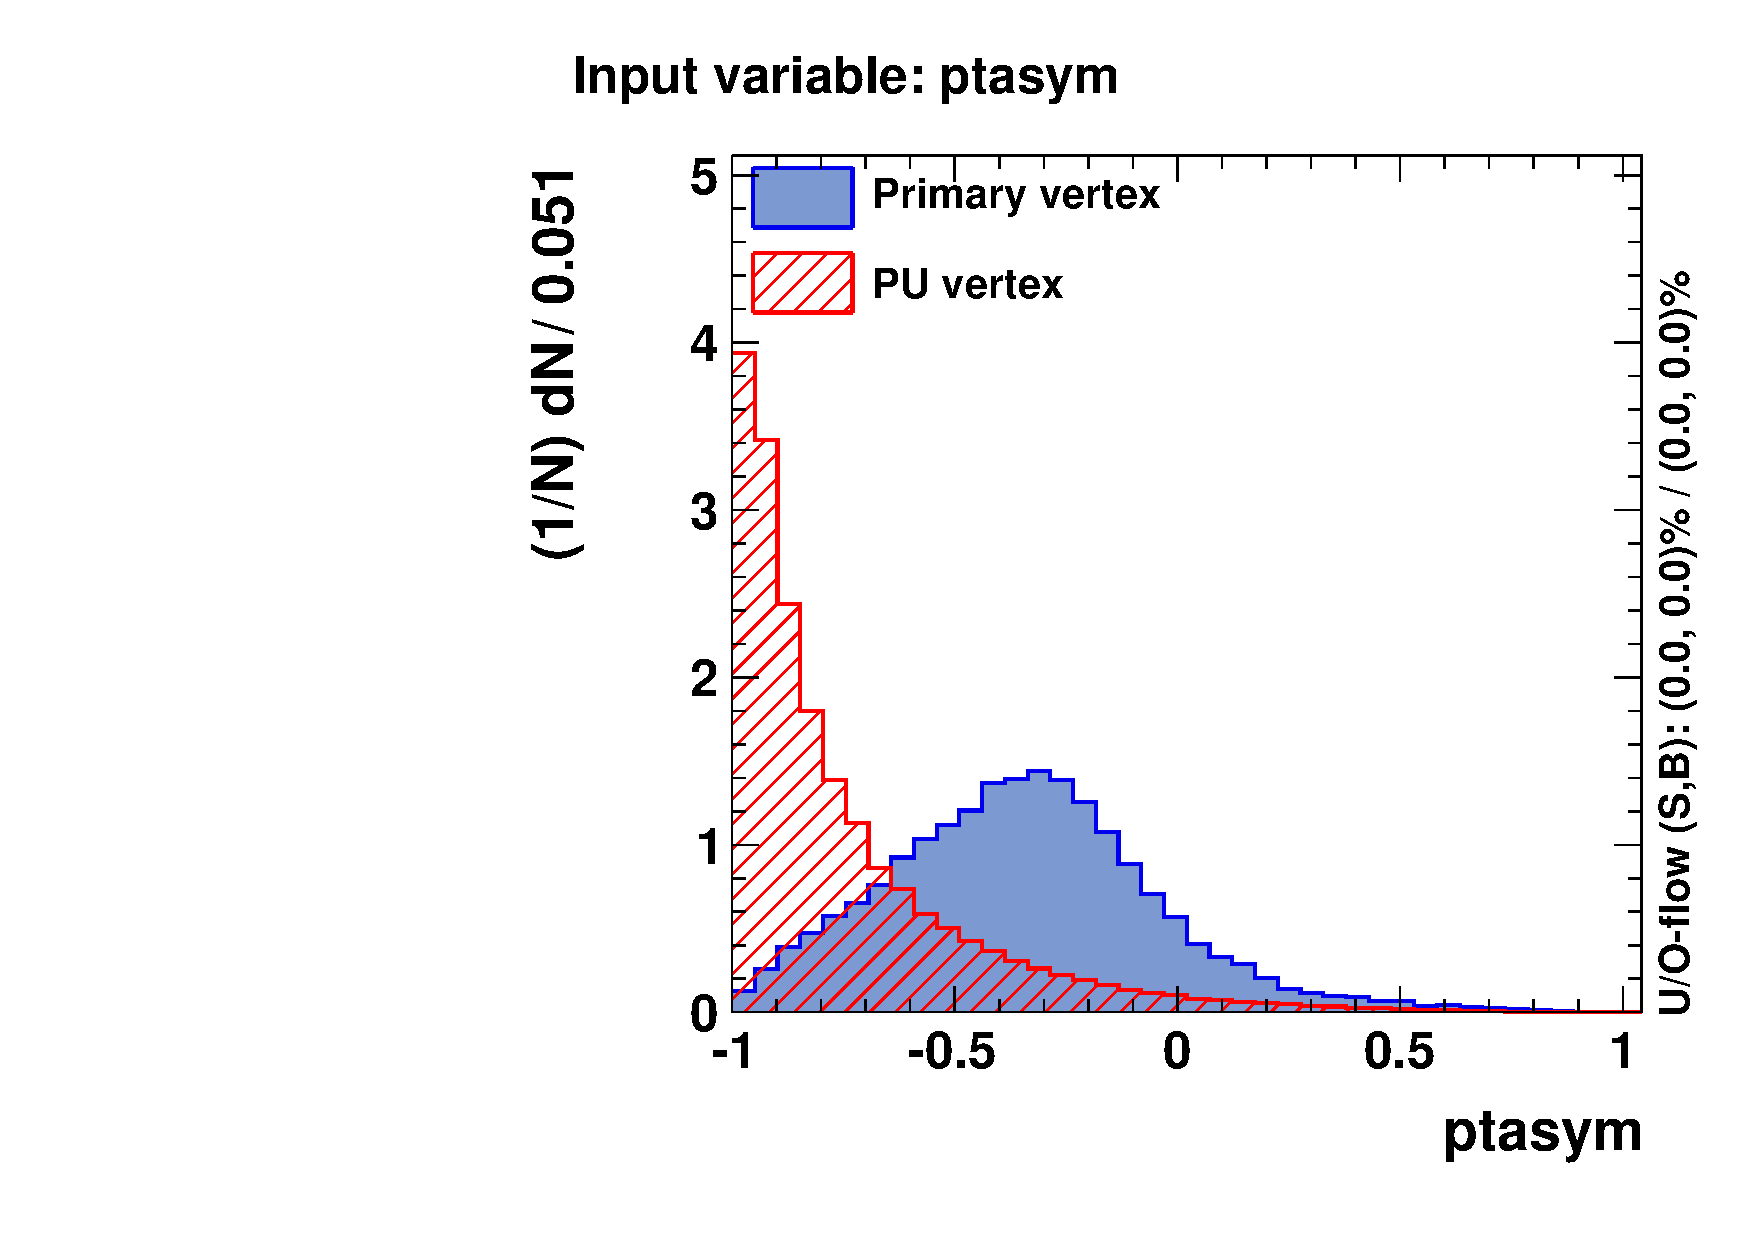
\includegraphics[width=0.48\textwidth]{ch3_comm_anal_comps/plots/vertex_bdt_input2.pdf}
  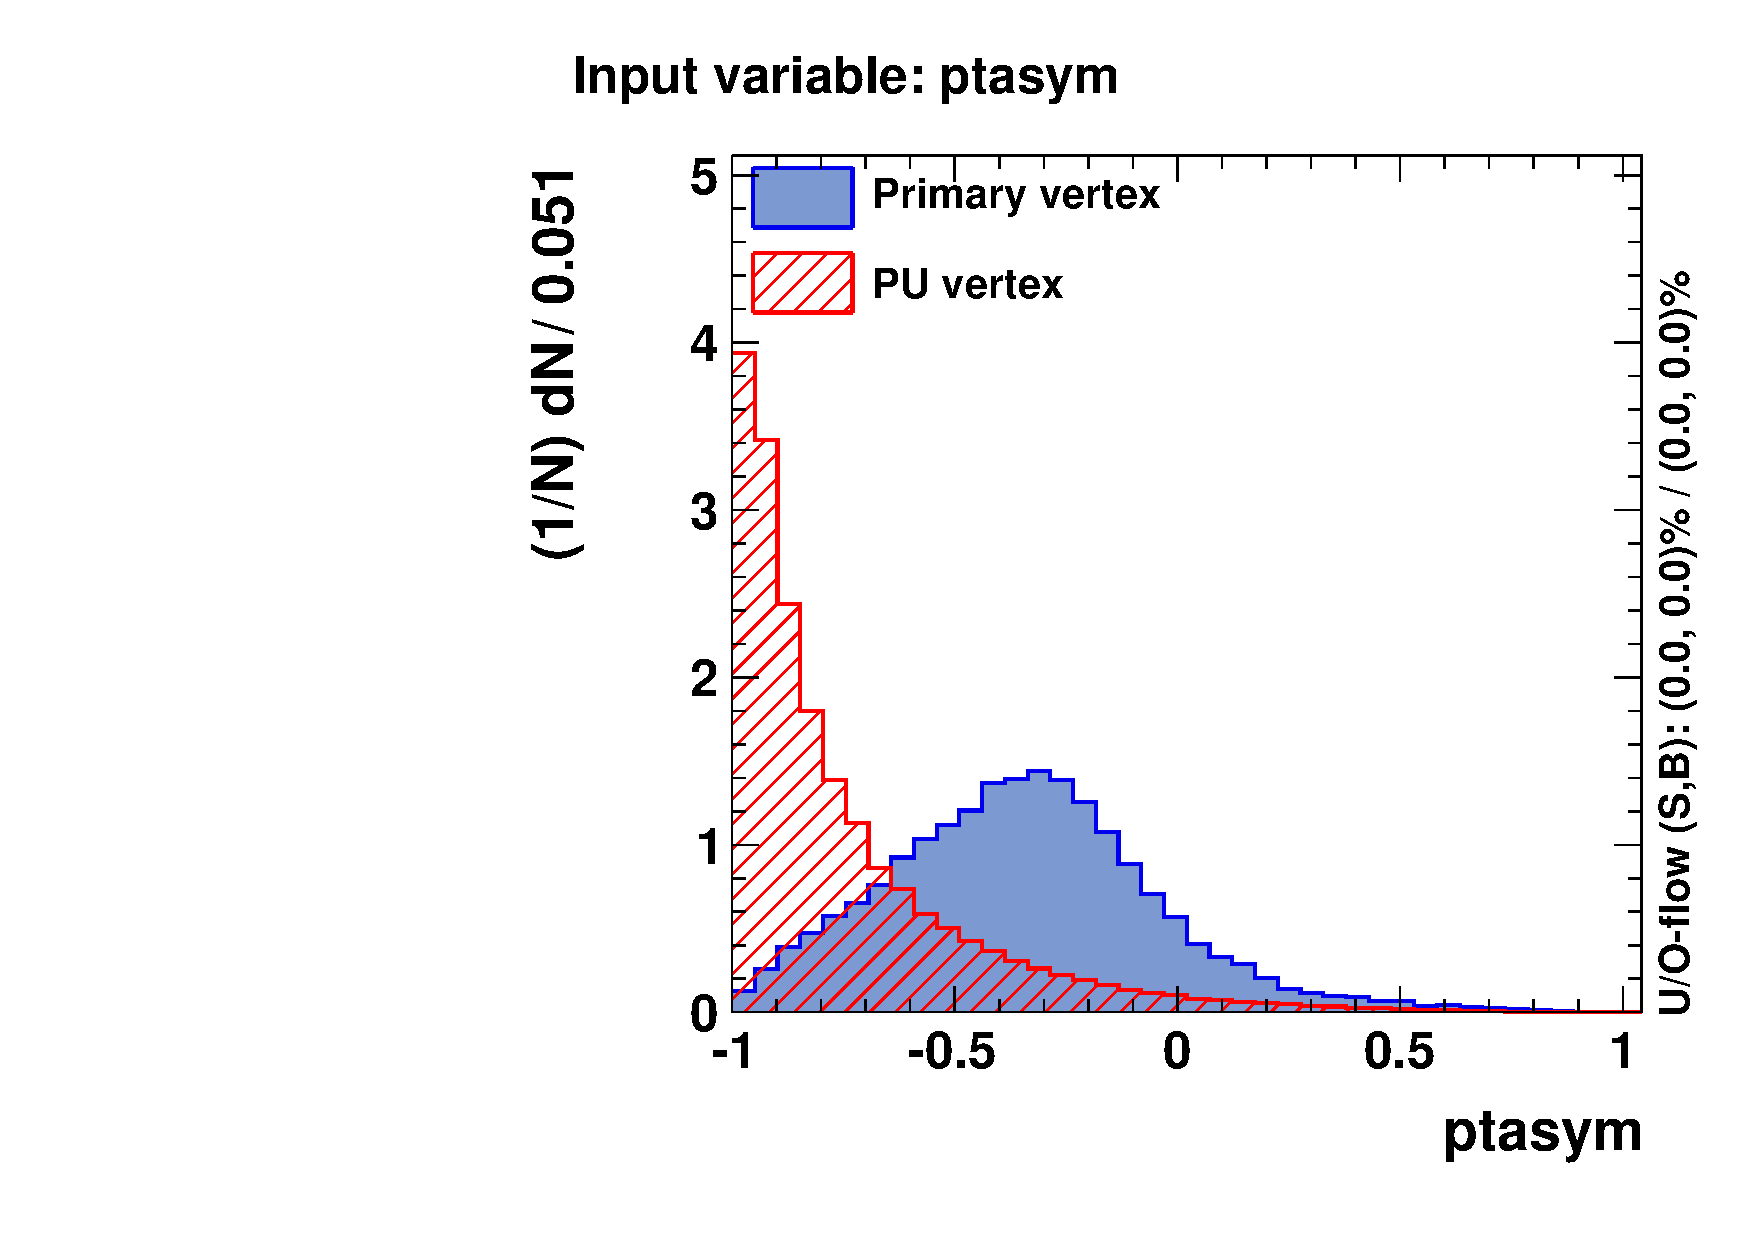
\includegraphics[width=0.48\textwidth]{ch3_comm_anal_comps/plots/vertex_bdt_input3.pdf}
  \caption{Distributions of the input variables for the vertex \BDT in the \MC \Hgg training (points) and test (filled) samples at 8TeV. Shown for the target primary vertex (blue histograms) and the background pileup vertices (red histograms). \red{Plots need updating, tidying and labelling correctly.}}
  \label{fig:vertex_bdt_inputs}
\end{figure}

\begin{figure}
  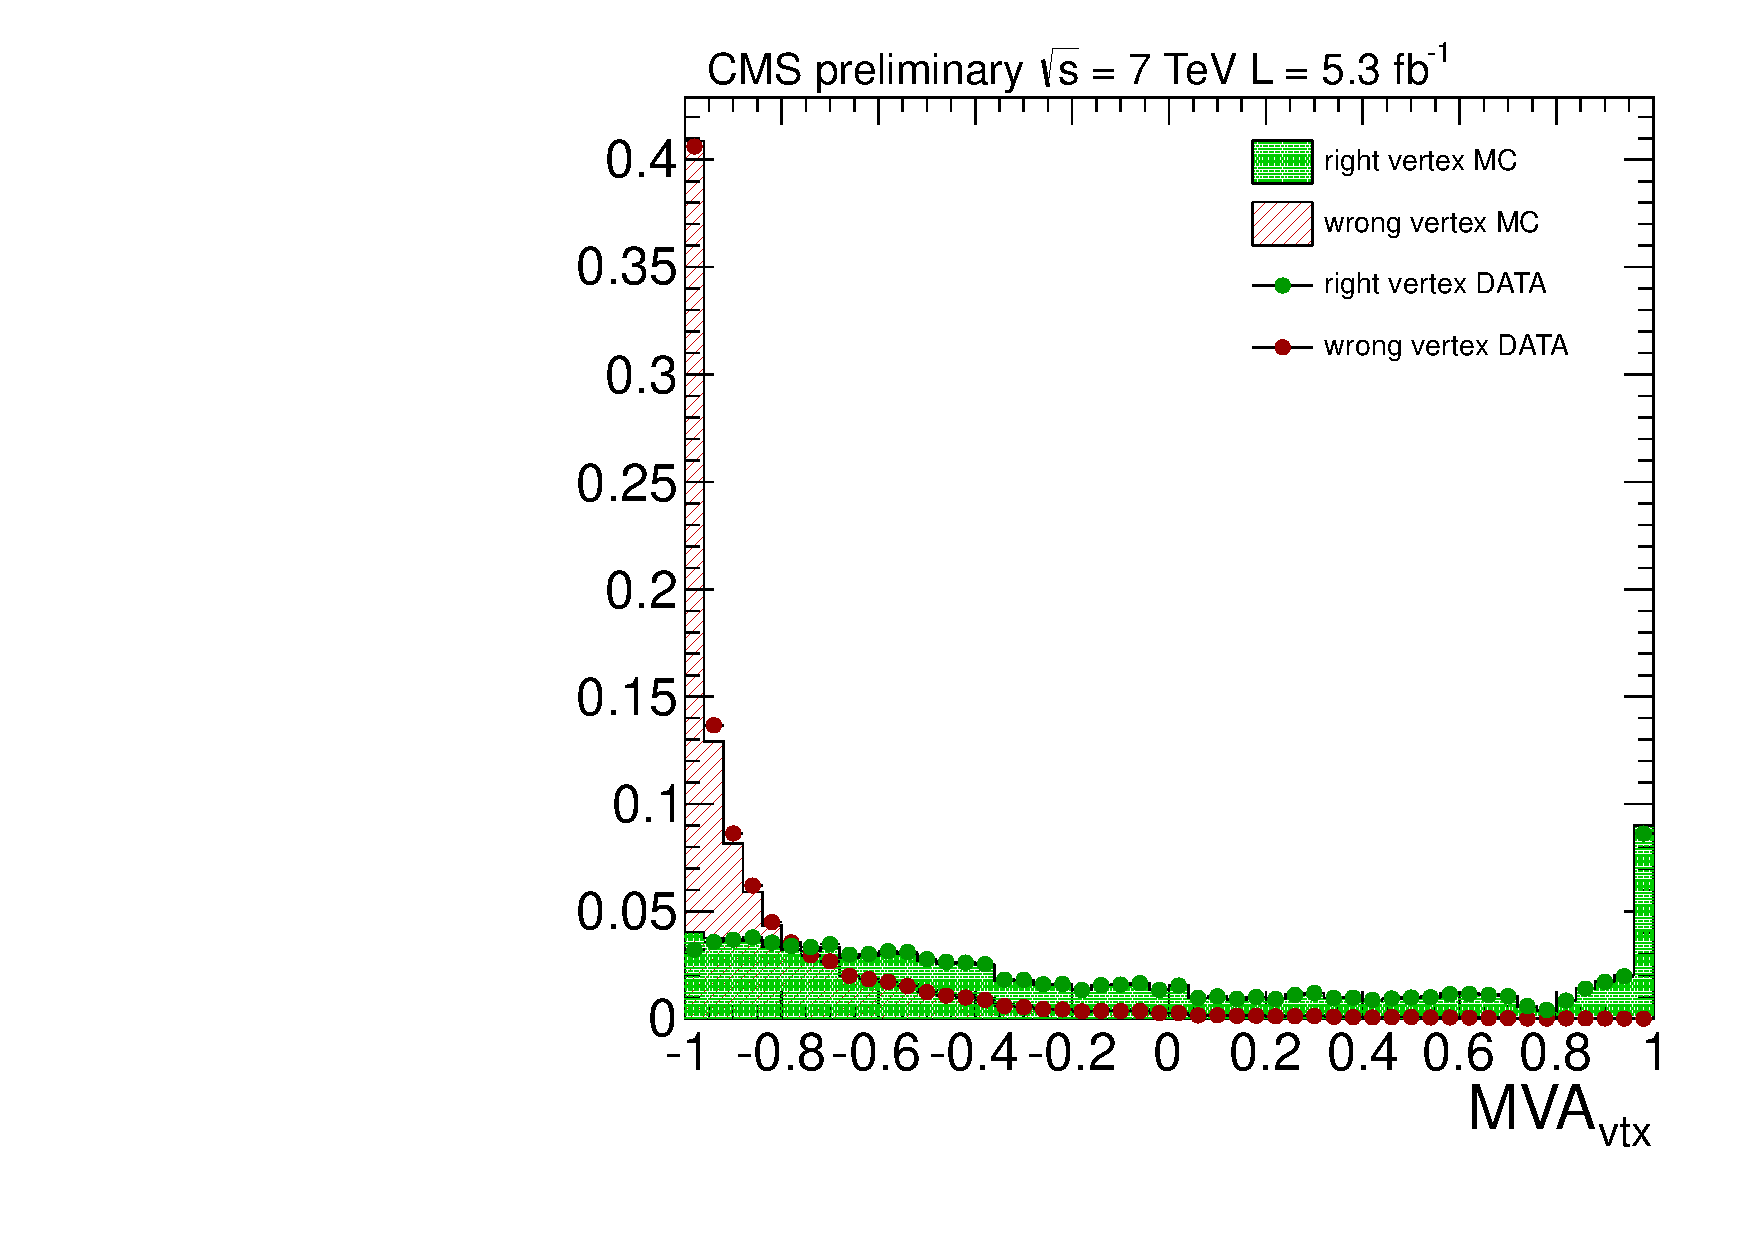
\includegraphics[width=0.48\textwidth]{ch3_comm_anal_comps/plots/vertex_bdt_output_7TeV.pdf}
  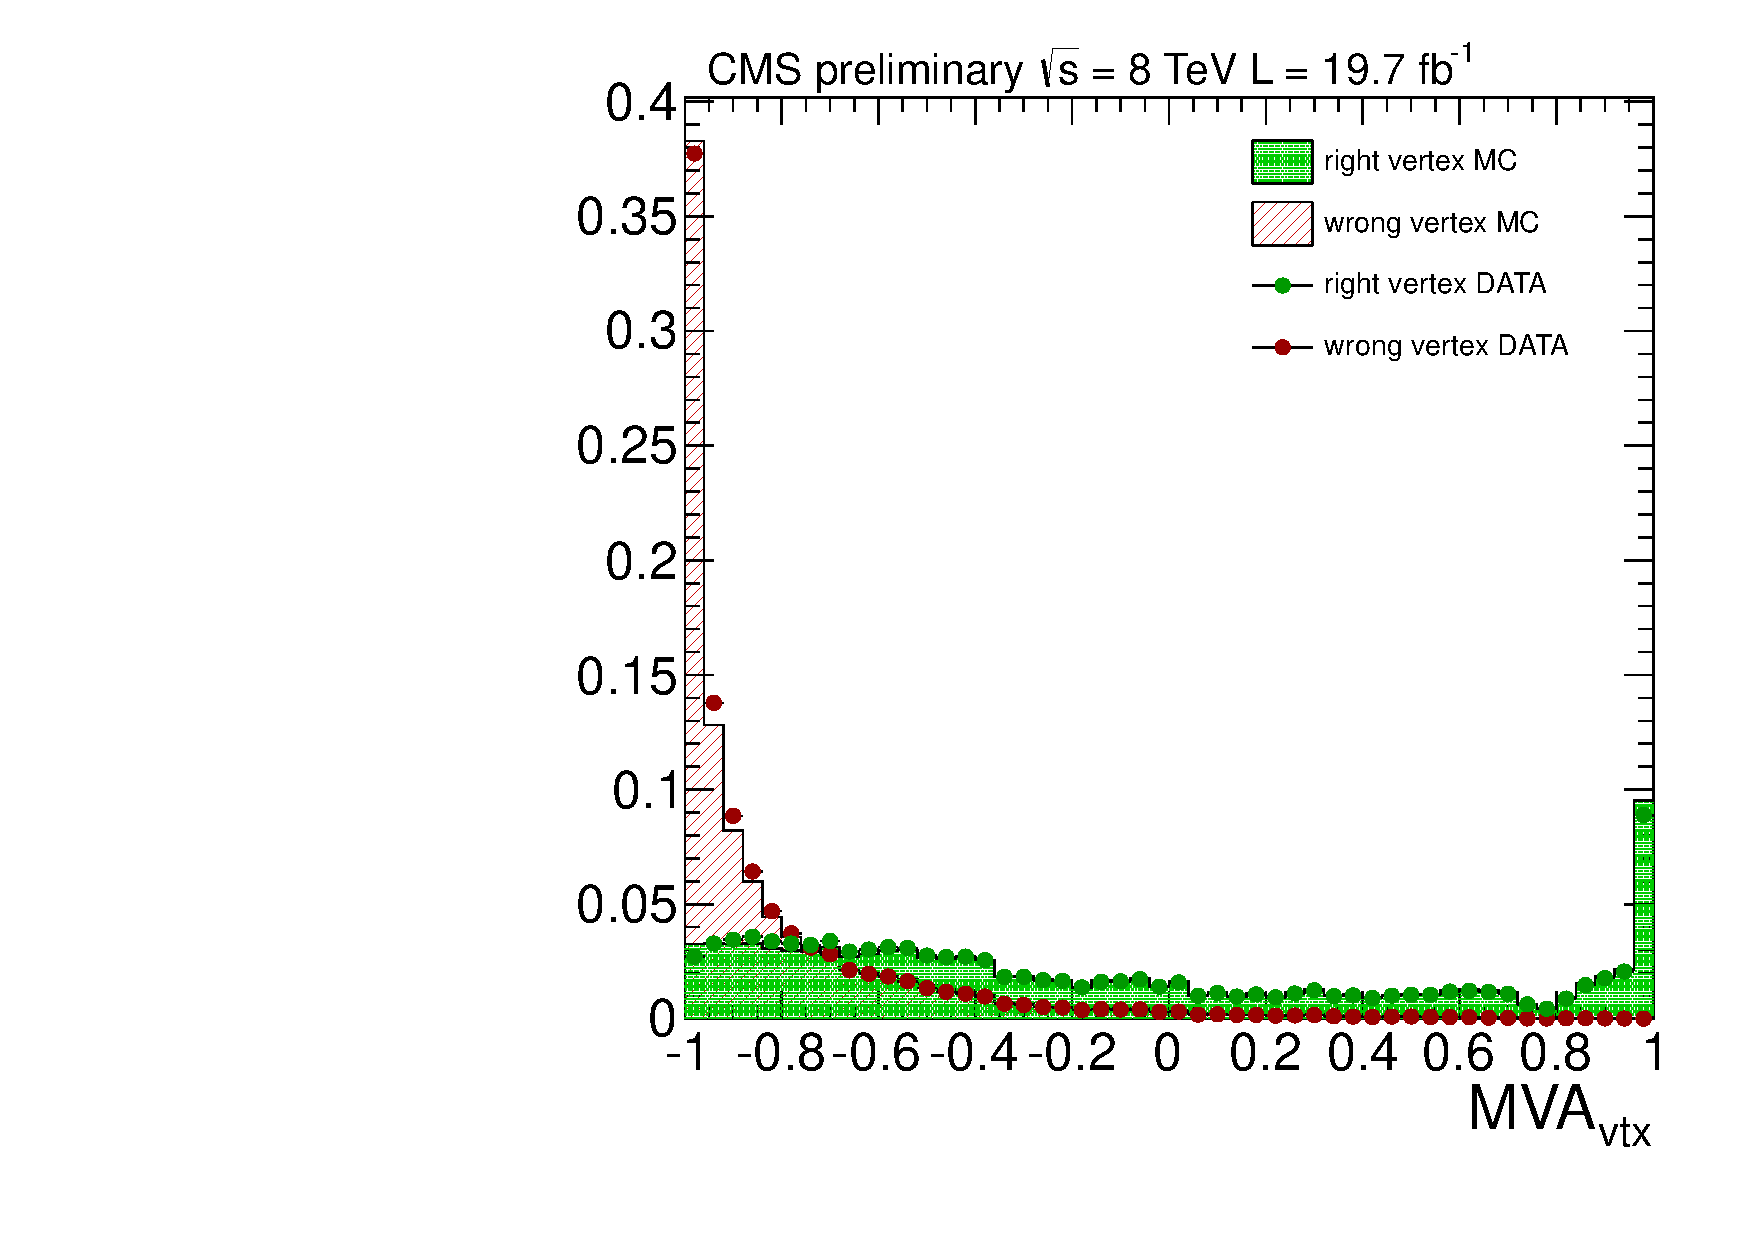
\includegraphics[width=0.48\textwidth]{ch3_comm_anal_comps/plots/vertex_bdt_output_8TeV.pdf}
  \caption{The vertex \BDT response for \Zmumu events in data (points) and MC (filled) for the primary vertex (green) and the background pileup vertices (red).}
  \label{fig:vertex_bdt_response}
\end{figure}

\begin{figure}
  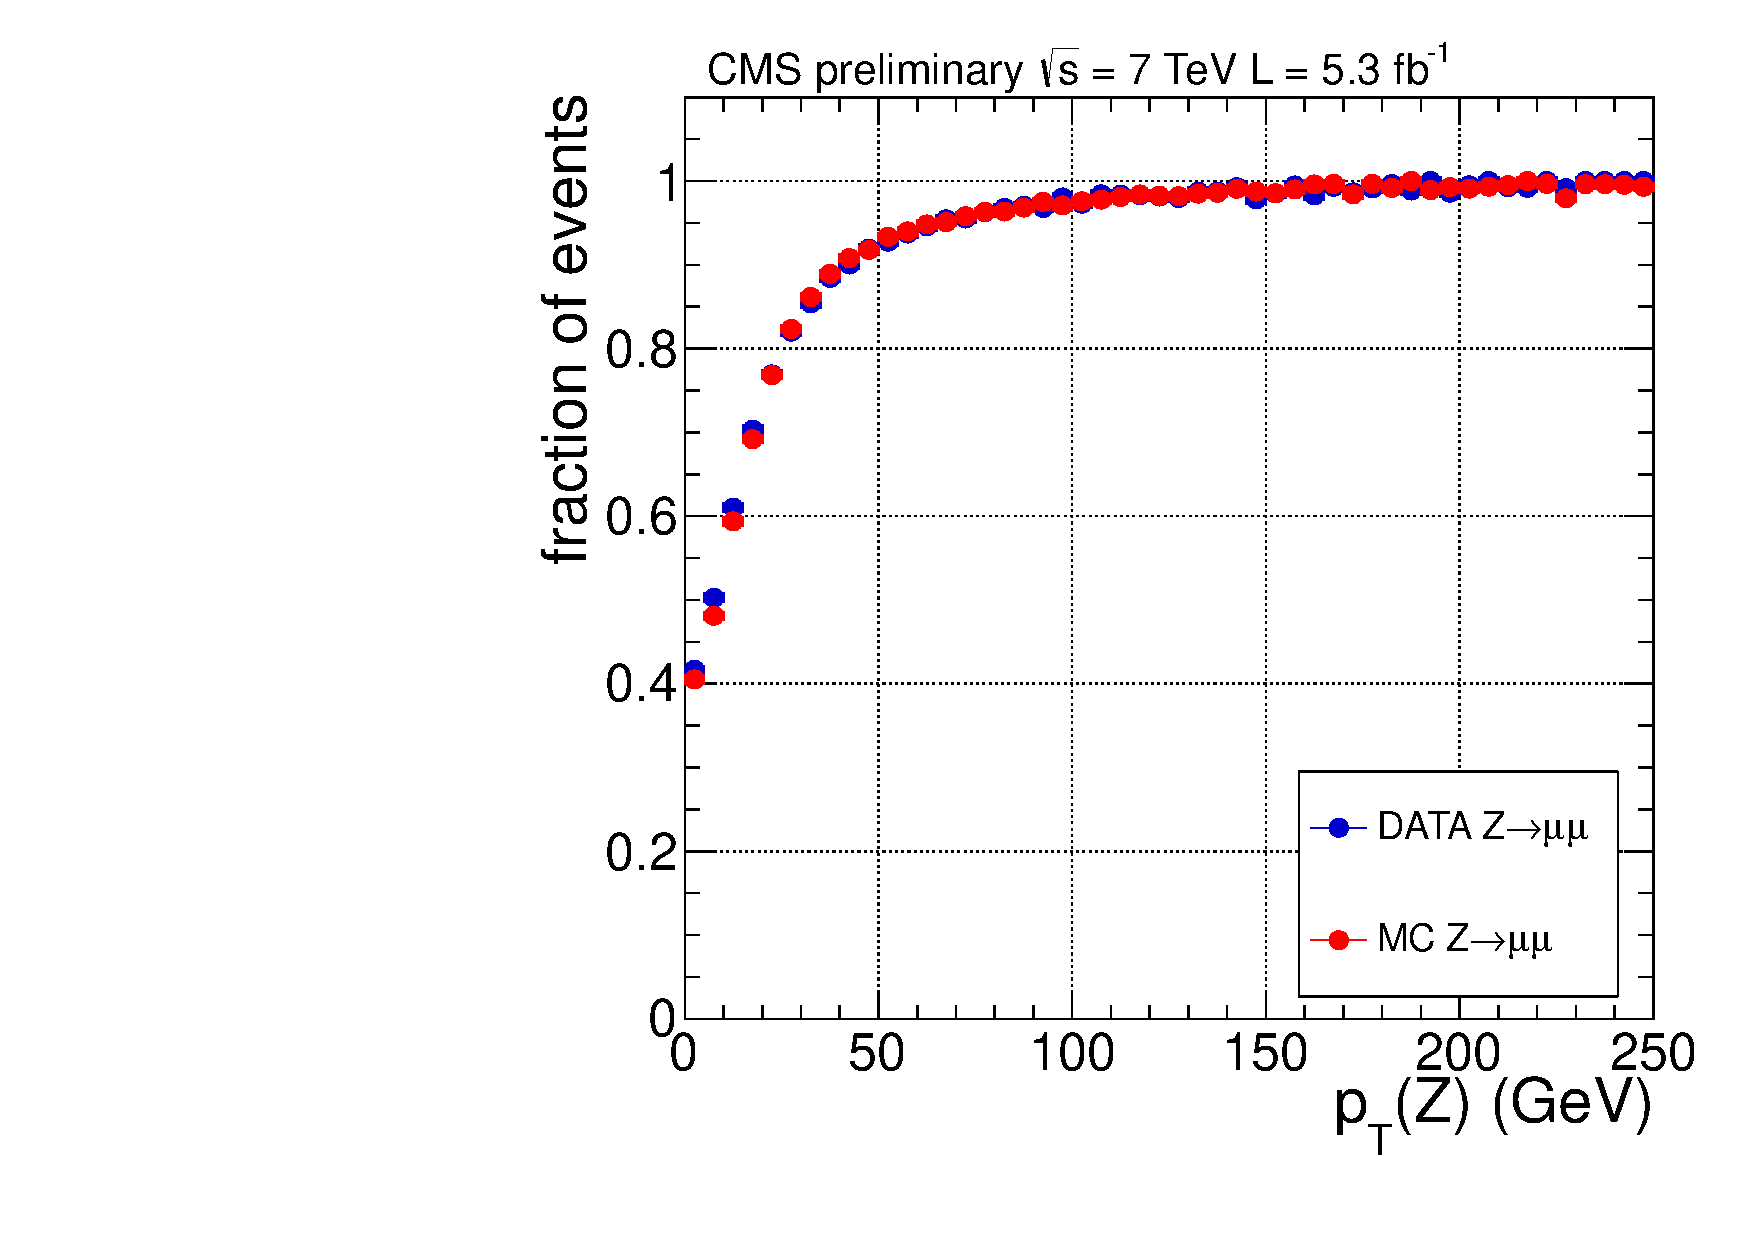
\includegraphics[width=0.48\textwidth]{ch3_comm_anal_comps/plots/vertex_bdt_efficiency_pt_7TeV.pdf}
  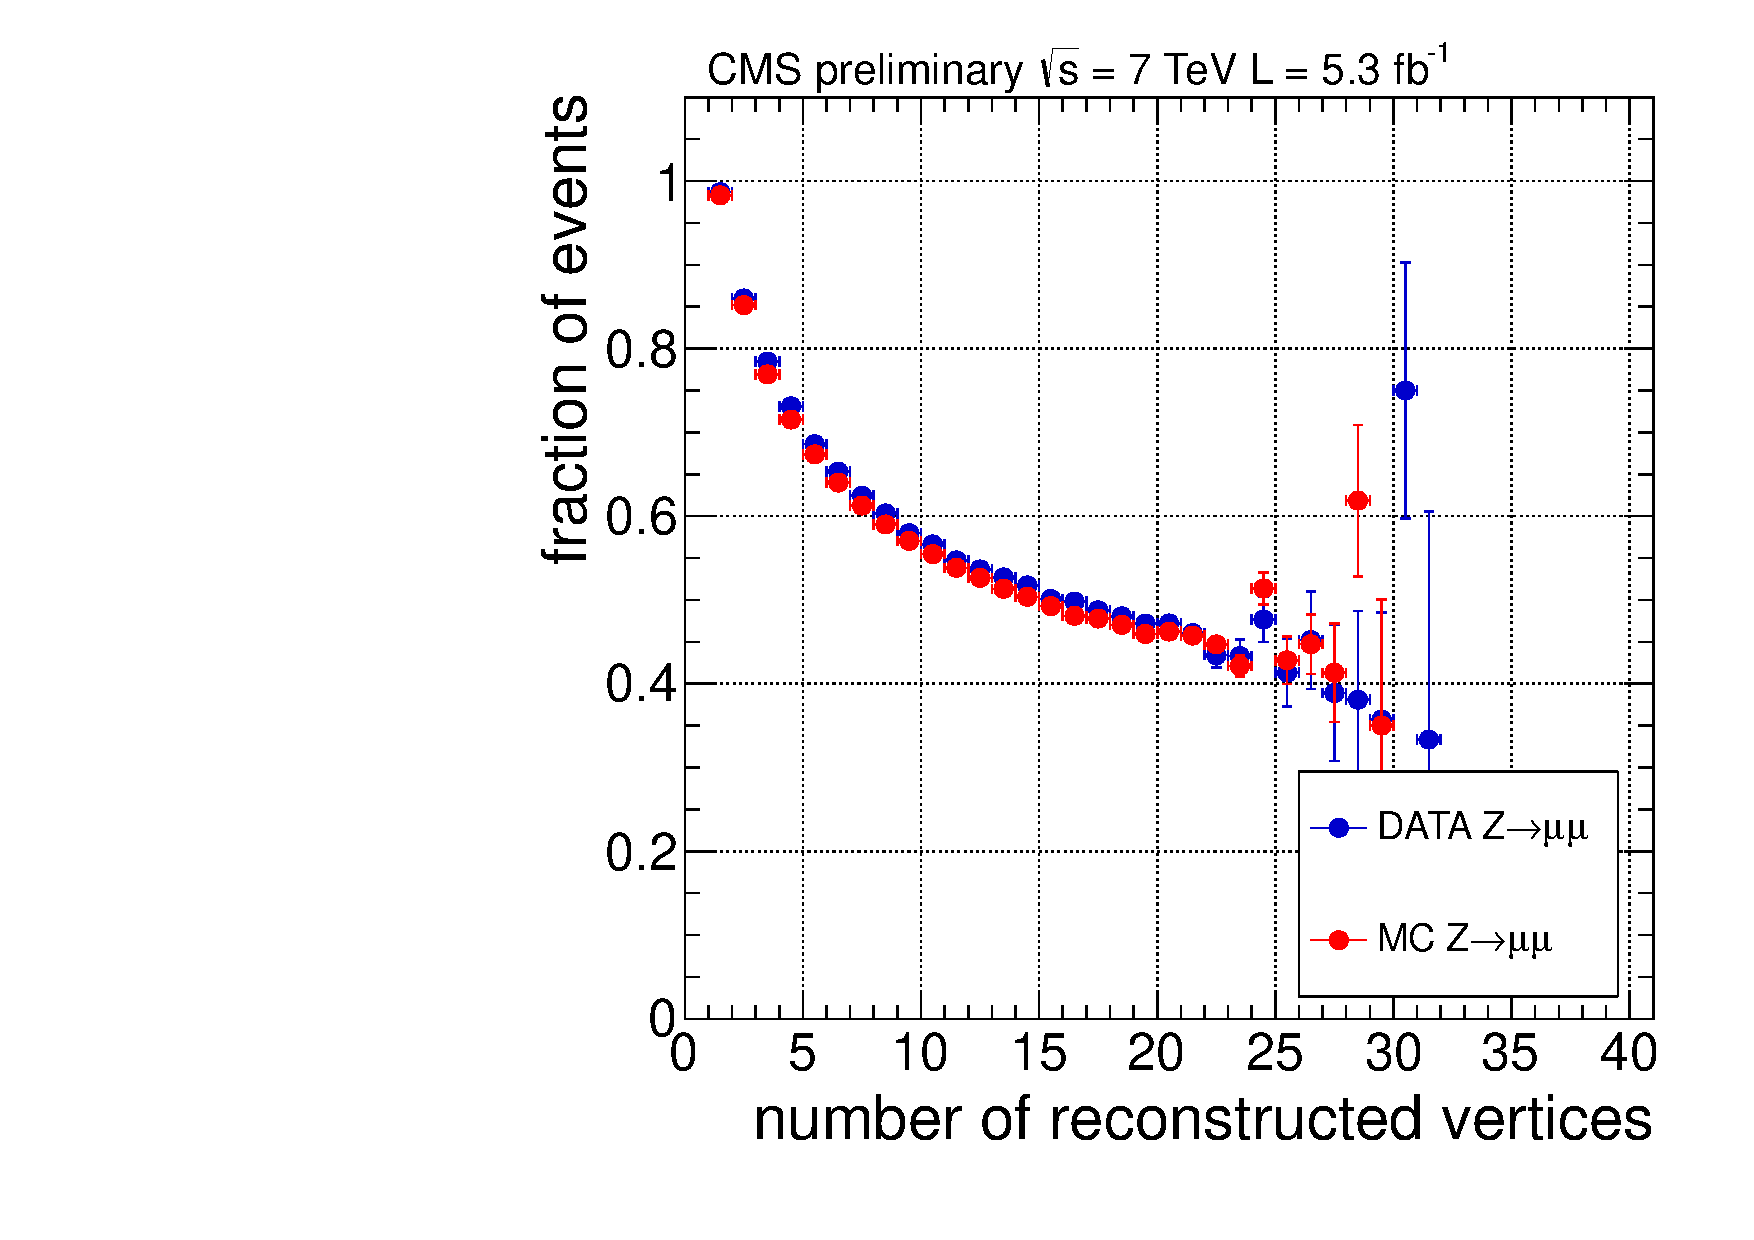
\includegraphics[width=0.48\textwidth]{ch3_comm_anal_comps/plots/vertex_bdt_efficiency_nvtx_7TeV.pdf} \\
  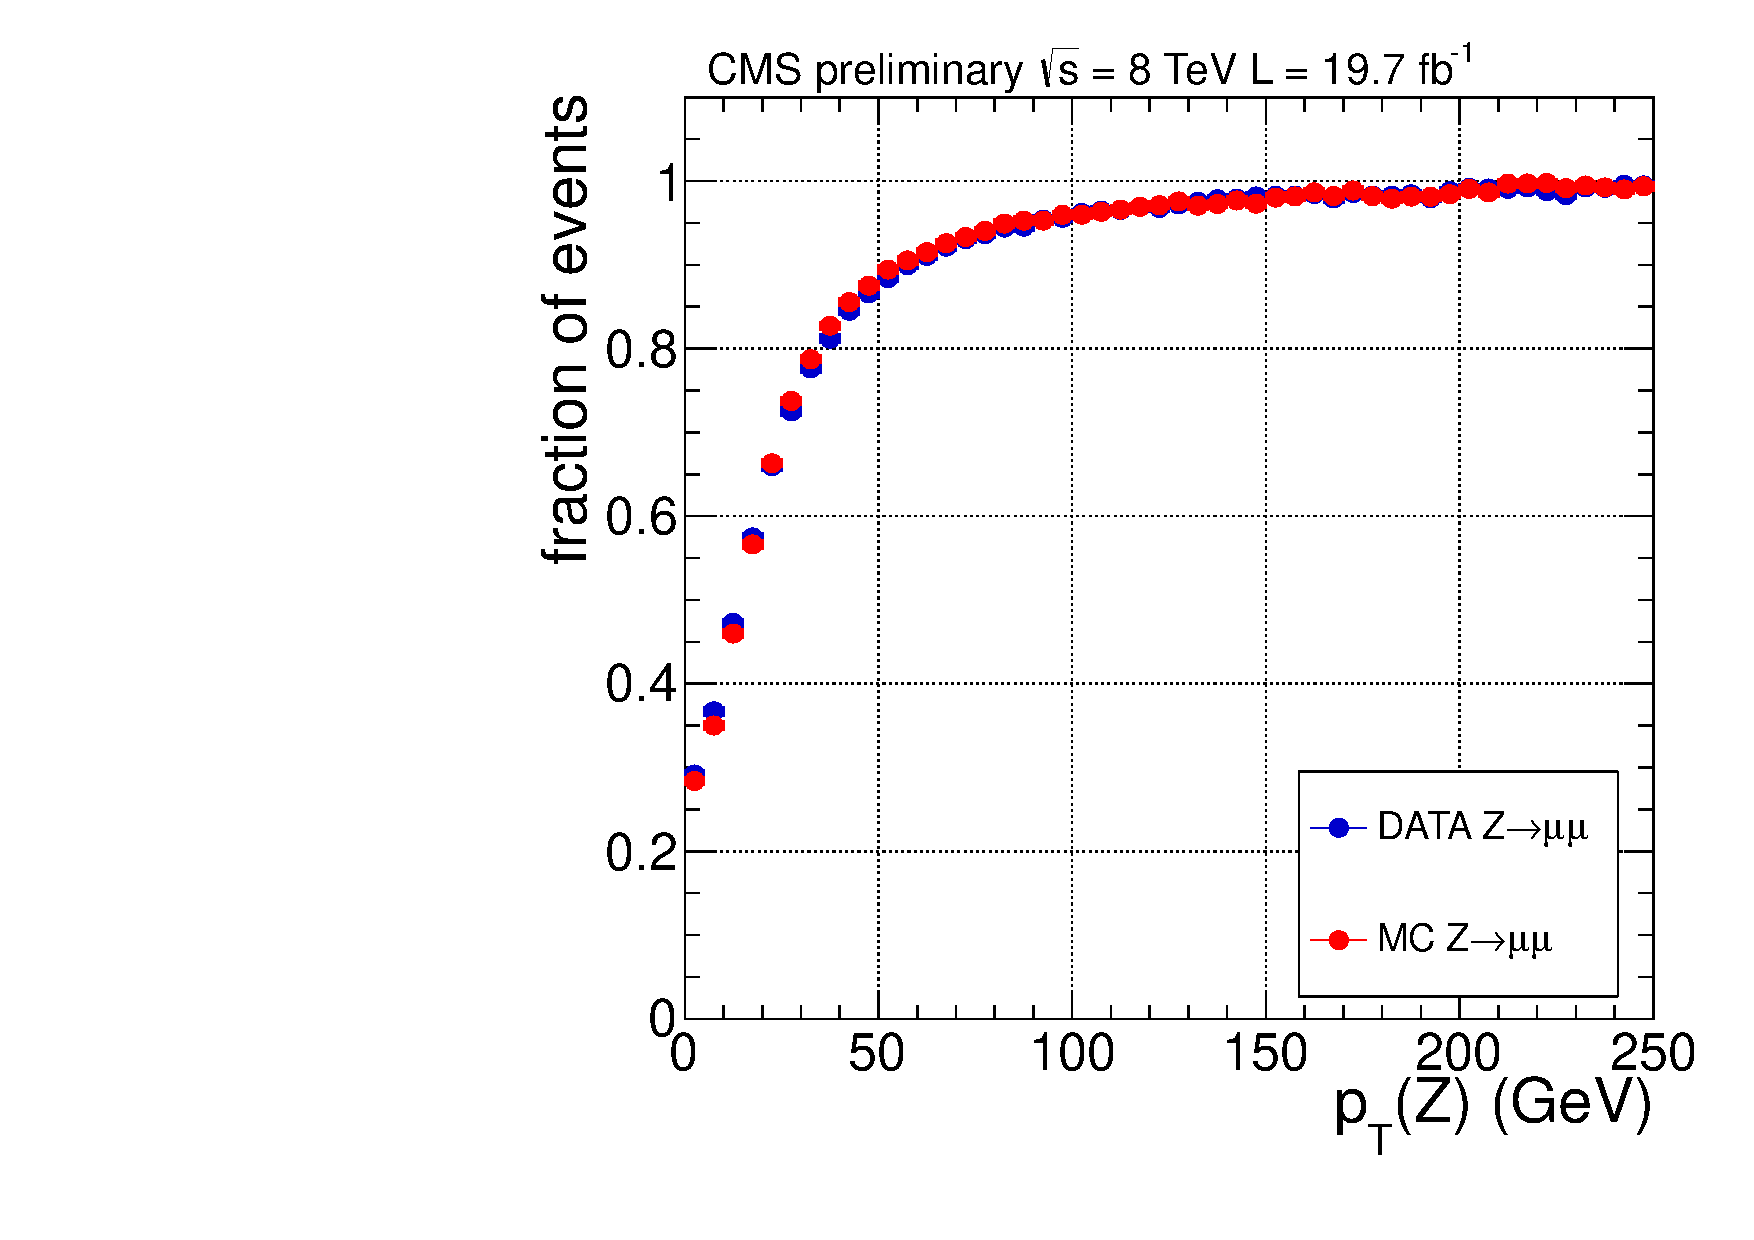
\includegraphics[width=0.48\textwidth]{ch3_comm_anal_comps/plots/vertex_bdt_efficiency_pt_8TeV.pdf}
  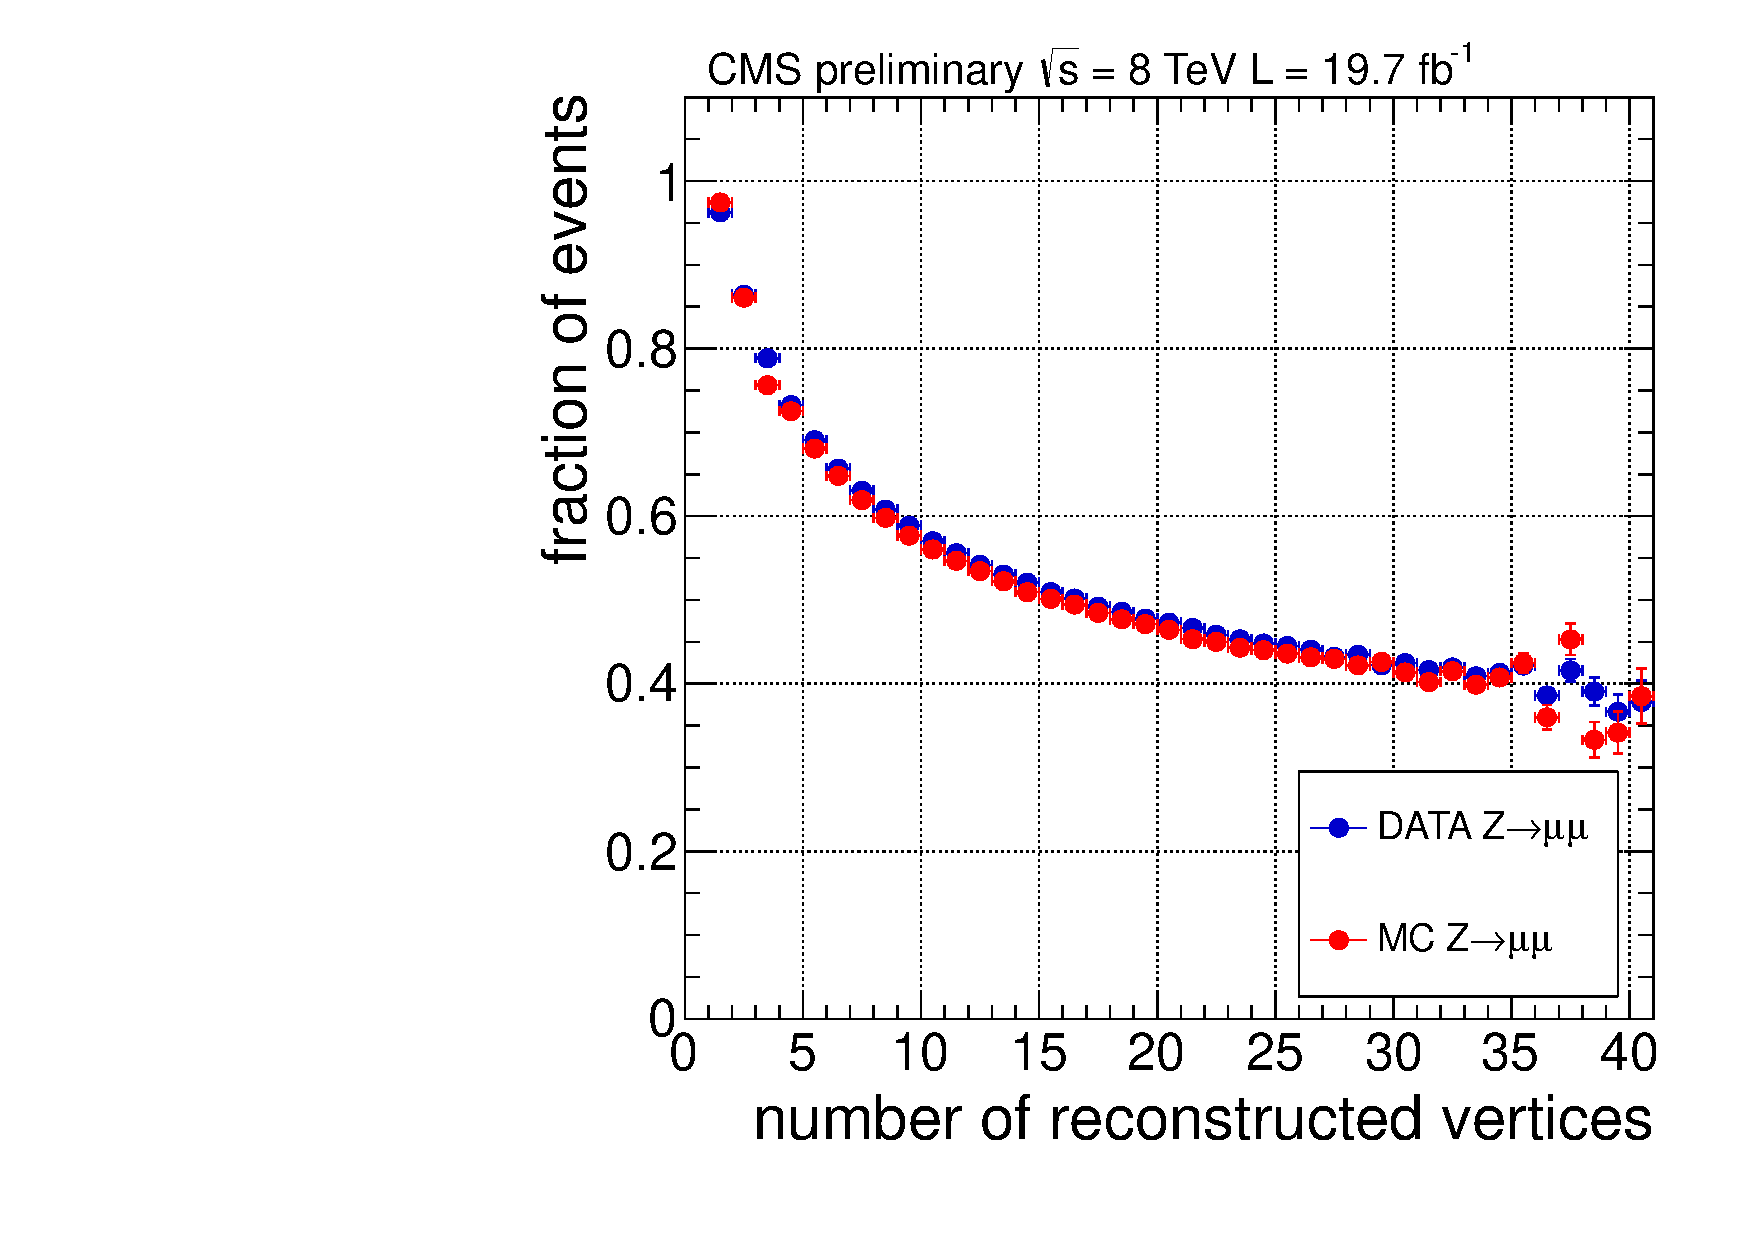
\includegraphics[width=0.48\textwidth]{ch3_comm_anal_comps/plots/vertex_bdt_efficiency_nvtx_8TeV.pdf} 
  \caption{The chosen vertex efficiency as measured in \Zmumu data and \MC as a function of $Z$ \pT (left) and number of reconstructed vertices (right) for the 7~TeV (top row) and 8~TeV (bottom row) data samples.}
  \label{fig:vertex_bdt_efficiency}
\end{figure}

\subsection{Estimating the per-event probability that the correct vertex is chosen}
\label{sec:bdt_prob}

The total efficiency of assigning the correct vertex using the method described in the preceeding section is at the level of 75\% during 2012 running conditions, where the correct vertex is defined as being within 10~mm of the true vertex. This means that for around 25\% of preselected events the mass resolution is dominated by the vertex resolution. Consequently, it is important to ascertain the probability that the chosen vertex is the correct one. An additional specific \BDT is constructed to address exactly this topic. The input variables used for this \BDT are:

\begin{itemize}
  \item The \pT of the diphoton system
  \item The number of vertices in each event
  \item The value of the per-vertex \BDT described above
  \item The $z$ distance, $\Delta z$, between the chosen vertex and the second and third choice vertices.
  \item The number of photon conversions used, either 0, 1 or 2.
\end{itemize}

There is a linear relation between the response of this \BDT and the correct vertex efficiency (or probability). This relation is demonstrated in Figure~\ref{fig:vertex_bdt_prob}. This relationship is fitted with a single parameter straight line and used to analytically obtain the per-event correct vertex probability given the response of this \BDT for a given event. Figure~\ref{fig:vertex_bdt_prob_efficiency} shows that this estimation reproduces the required vertex efficiency as a function of Higgs \pT and number of reconstructed vertices.

\begin{figure}
  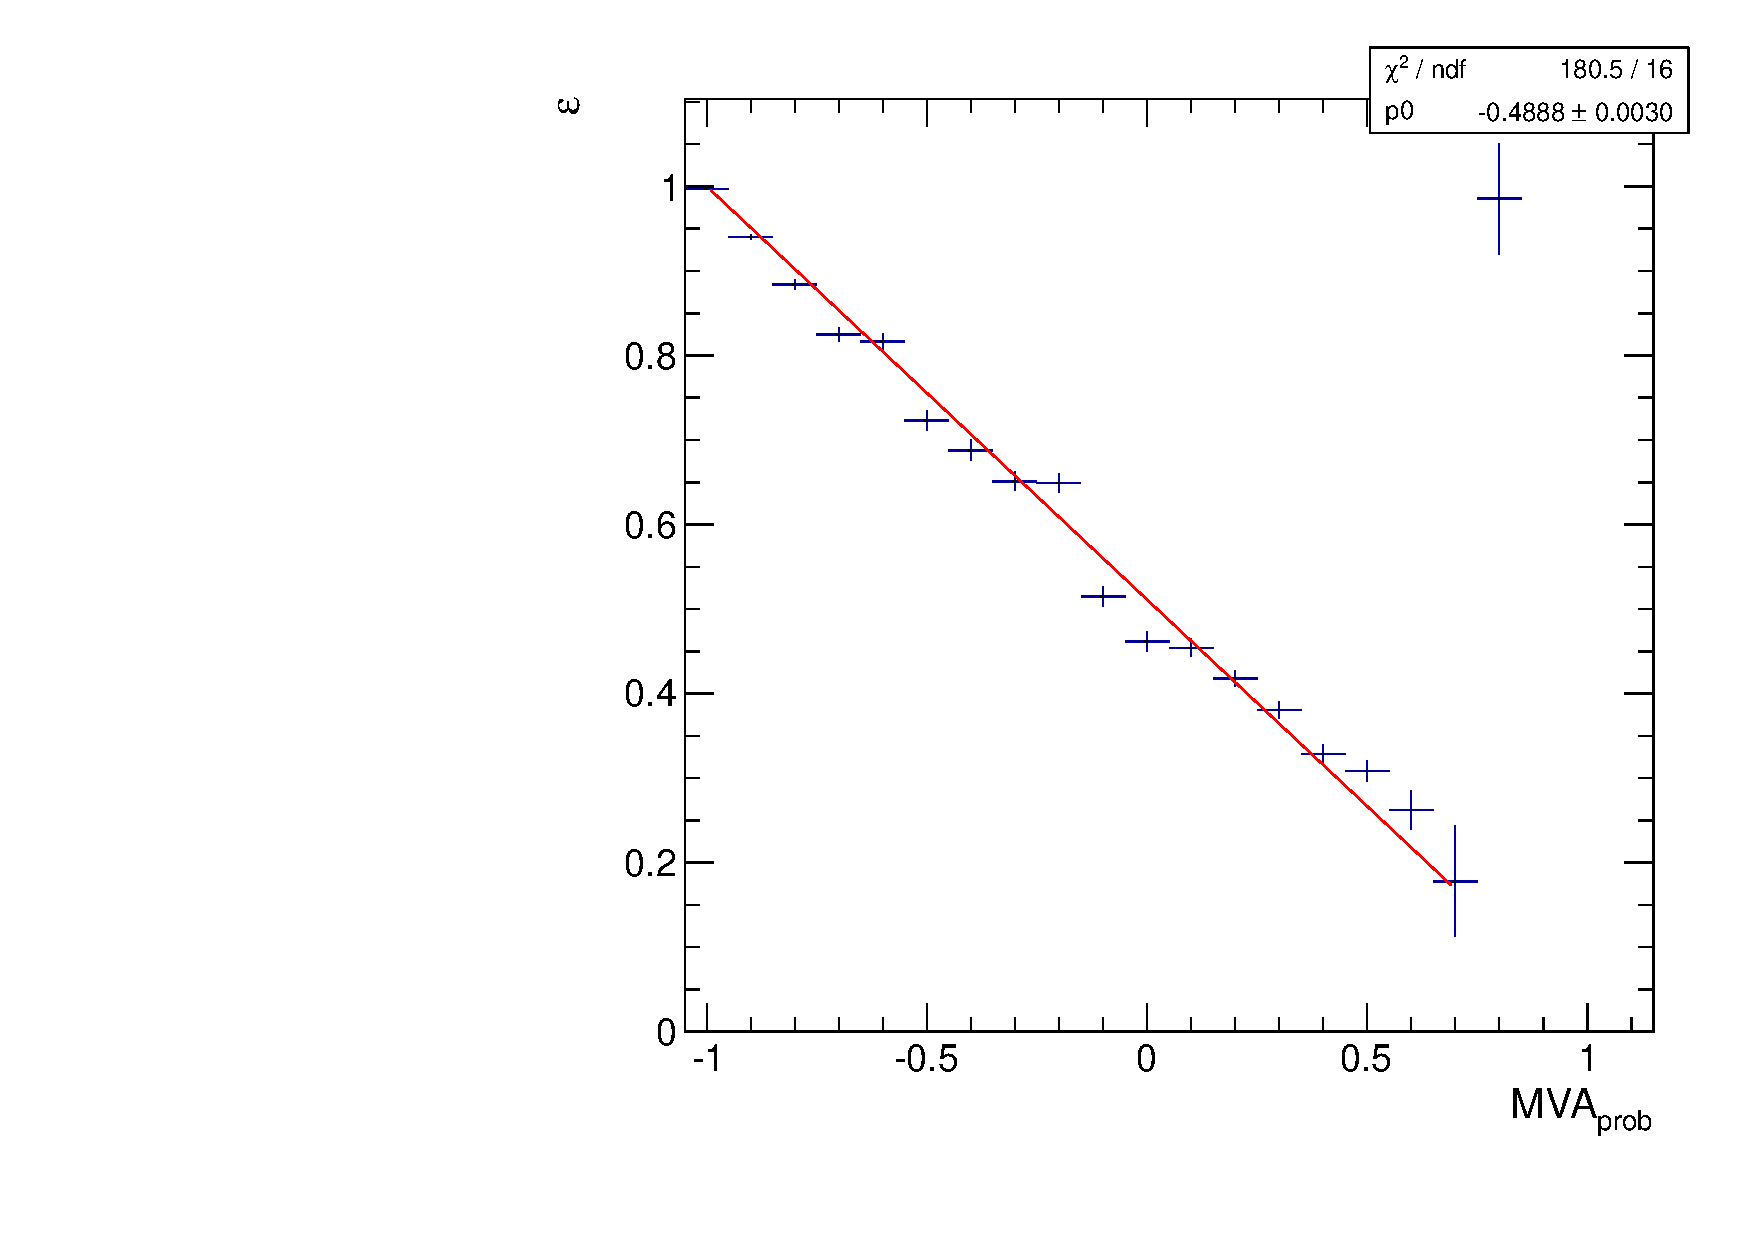
\includegraphics[width=0.48\textwidth]{ch3_comm_anal_comps/plots/vertex_bdt_prob.pdf}
  \caption{A demonstration of the linearity relation between the per-event vertex probability \BDT output distribution and the correct vertex probability}
  \label{fig:vertex_bdt_prob}
\end{figure}

\begin{figure}
  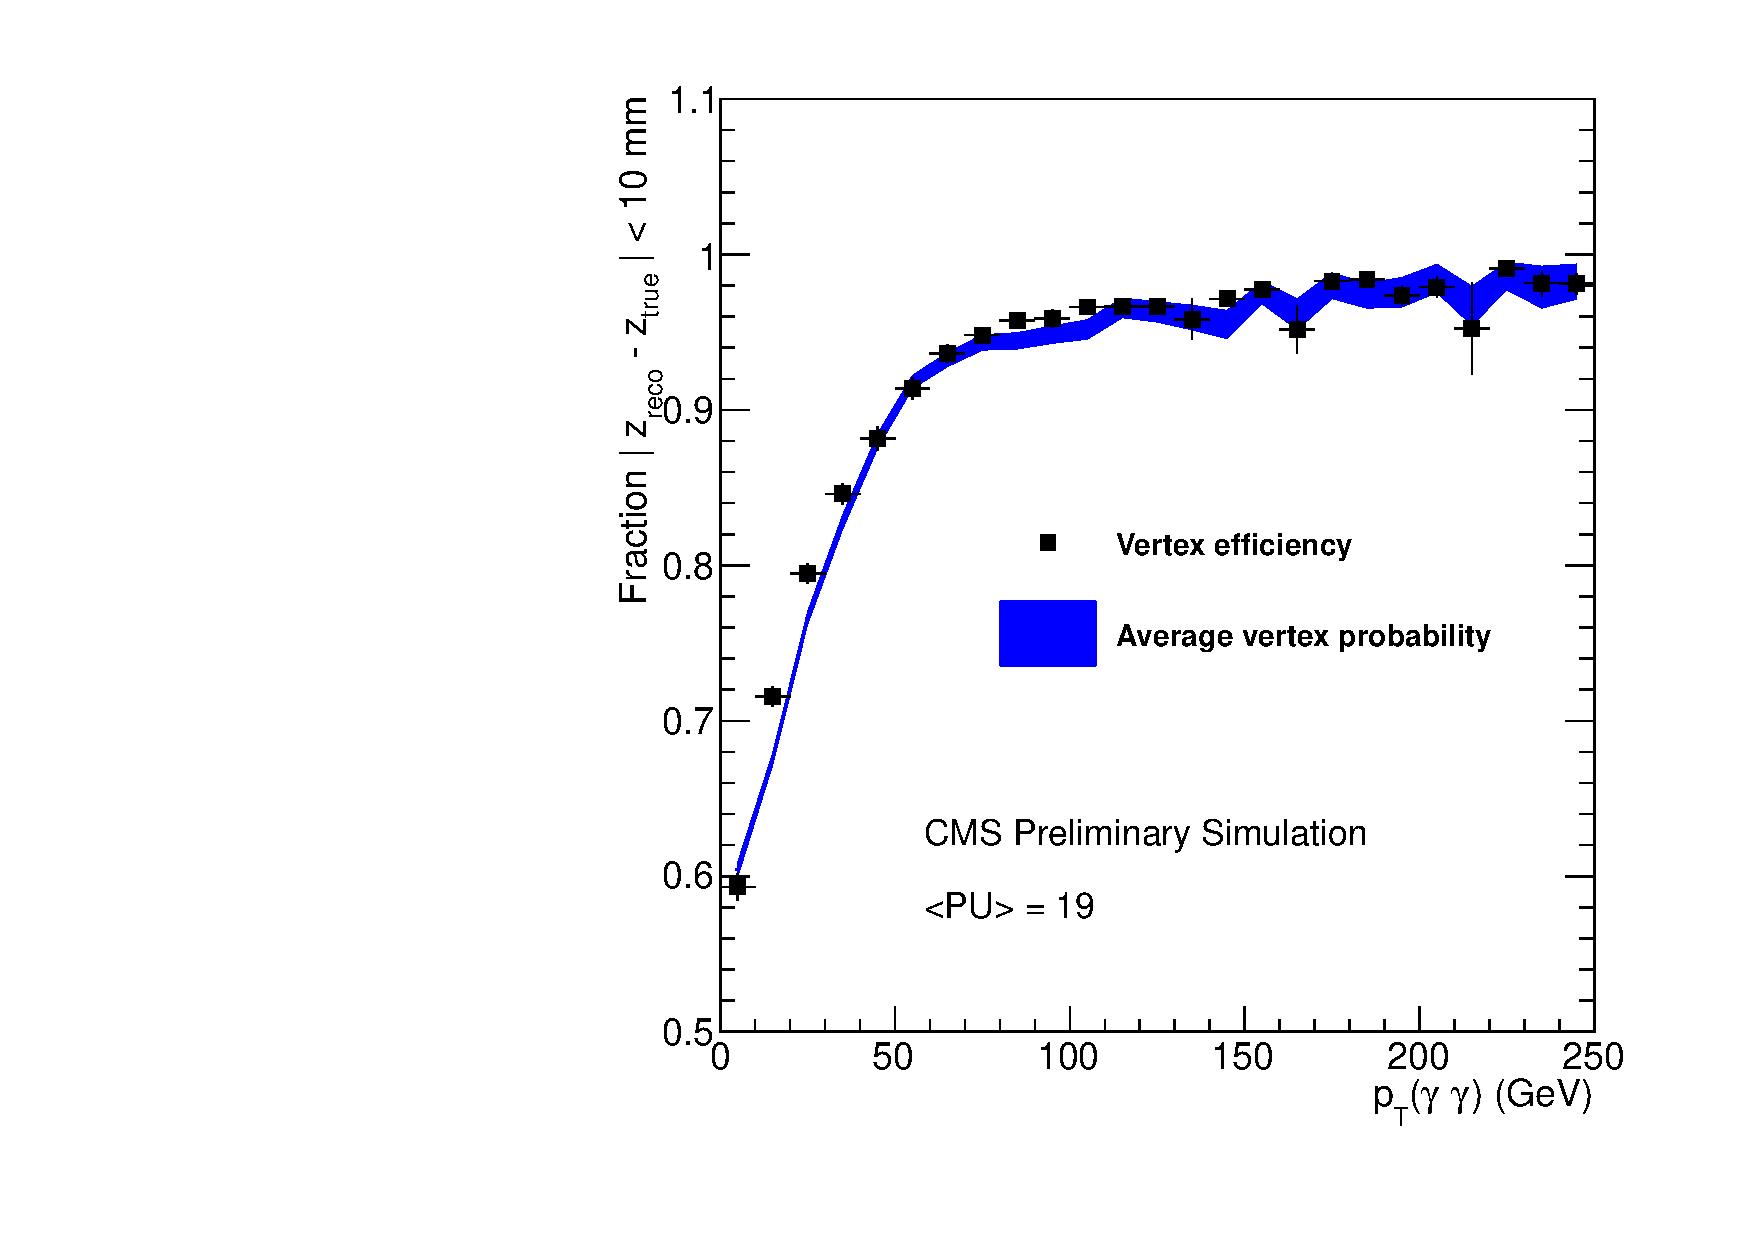
\includegraphics[width=0.48\textwidth]{ch3_comm_anal_comps/plots/vertex_bdt_prob_efficiency_pt.pdf}
  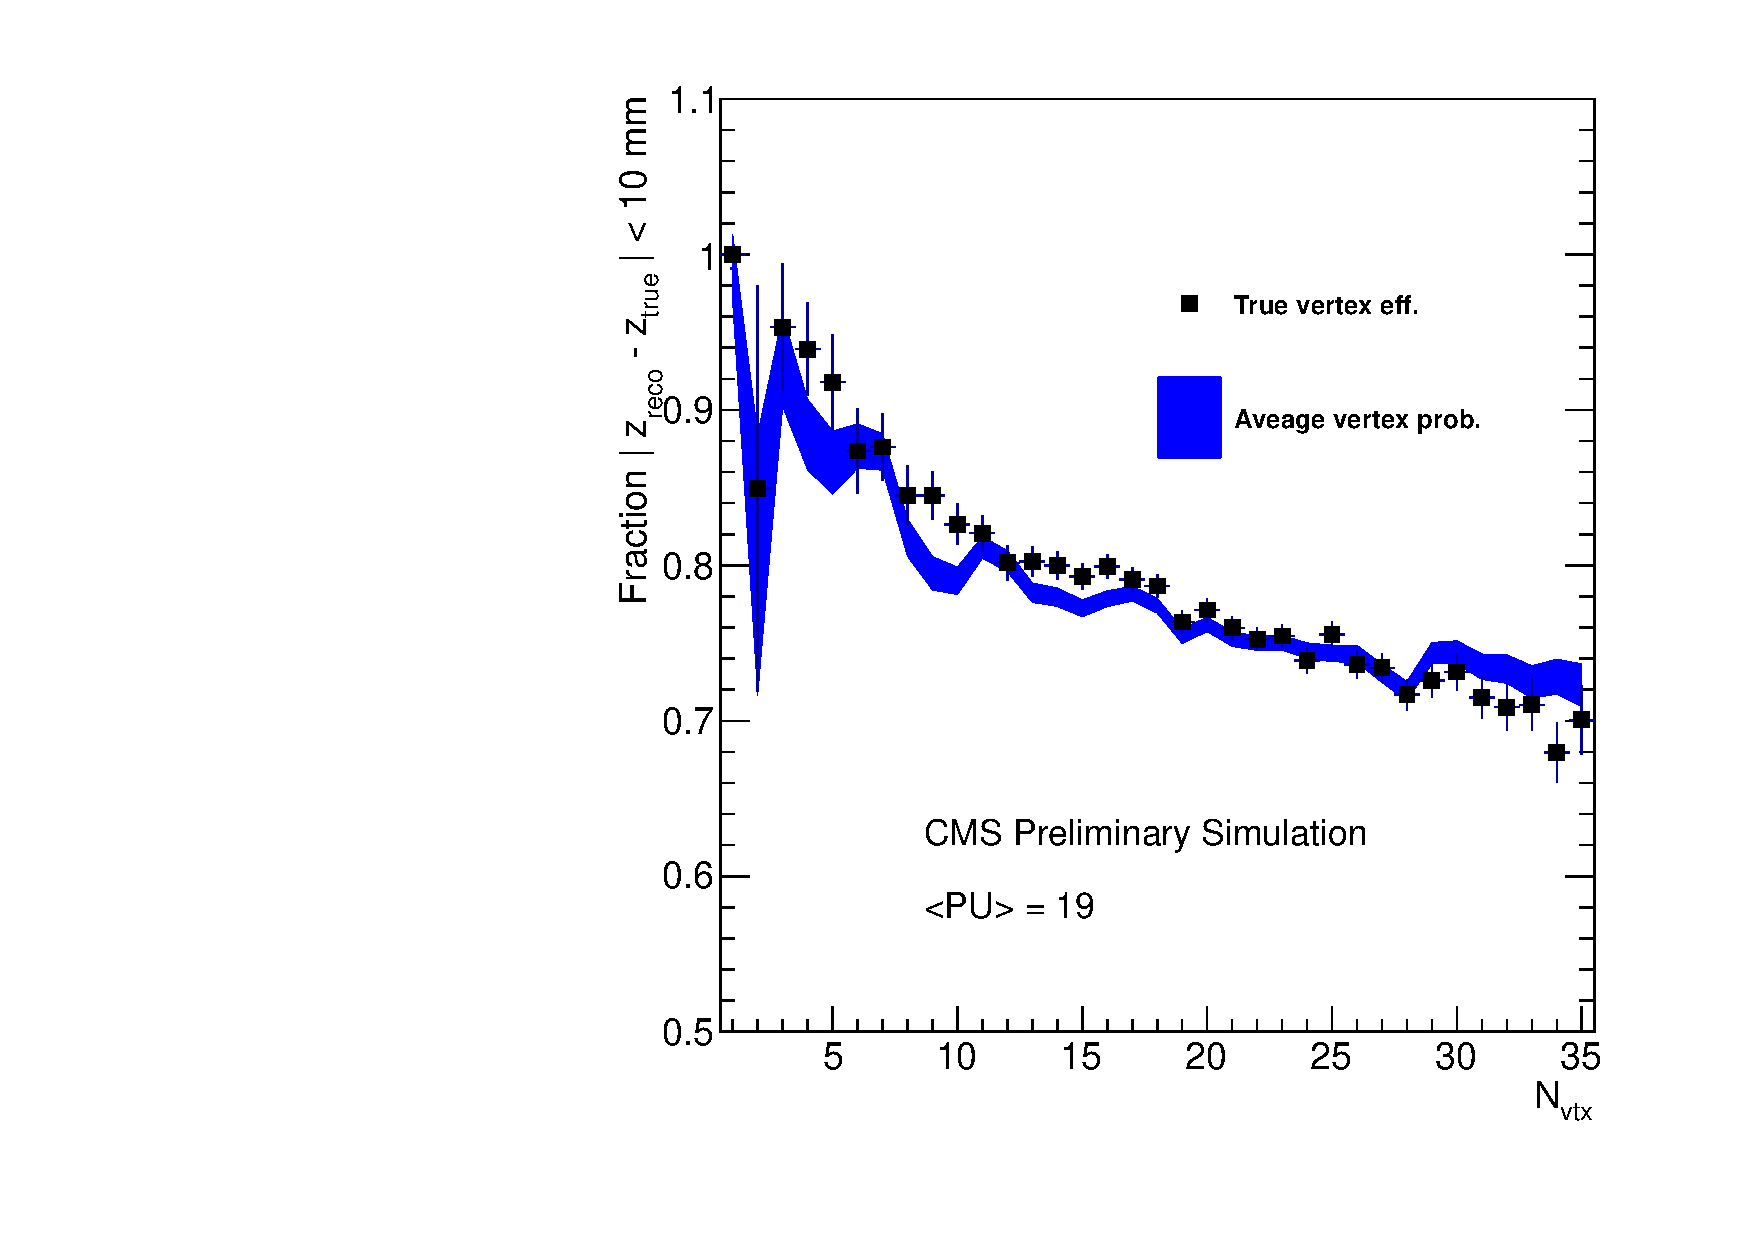
\includegraphics[width=0.48\textwidth]{ch3_comm_anal_comps/plots/vertex_bdt_prob_efficiency_nvtx.pdf}
  \caption{A comparison of the true vertex efficiency (black points) and the average vertex probability (blue band) a statistically independent \MC Higgs sample simulated with 2012 running conditions.}
  \label{fig:vertex_bdt_prob_efficiency}
\end{figure}

\section{Event preselection}
\label{sec:photon_presel}

\section{Using \Zee decays for validation and efficiency measurements}
\label{sec:zee}

